\documentclass{article}
\usepackage[style=ieee]{biblatex}


\bibliography{article}

\addbibresource{\jobname.bib}
%\AtEveryBibitem{\printfield{note}\clearfield{note}\item}


\usepackage{subcaption}
\usepackage[margin=1in]{geometry}
\usepackage{amsmath}
\usepackage[table]{xcolor}% http://ctan.org/pkg/xcolor
\usepackage{tikz}
\usetikzlibrary{angles}
\usetikzlibrary{arrows.meta}
\usetikzlibrary{automata}
\usetikzlibrary{calc}
\usetikzlibrary{chains}
\usetikzlibrary{decorations.pathreplacing}
\usetikzlibrary{positioning}
\usetikzlibrary{quotes}
\usepackage{graphicx} % Required for inserting images
\usepackage[T1]{fontenc}
\usepackage{beramono}
\usepackage{courier}
\usepackage{listings}
\usepackage{xpatch}
\usepackage{realboxes}
\usepackage{titlesec}
\usepackage{xcolor}
\usepackage{minted}
\usepackage{nicematrix}
\usepackage{collcell}
\usepackage{varwidth}
\usepackage{booktabs}
\usepackage{float}
\usepackage{svg}

\definecolor{LightGray}{gray}{0.97}


\setcounter{secnumdepth}{4}


\titleformat{\paragraph}
{\normalfont\normalsize\bfseries}{\theparagraph}{1em}{}
\titlespacing*{\paragraph}
{0pt}{3.25ex plus 1ex minus .2ex}{1.5ex plus .2ex}


\lstdefinelanguage{none}{
  identifierstyle=
}

\definecolor{mygreen}{rgb}{0,0.8,0}
\definecolor{mygray}{rgb}{0.5,0.5,0.5}
\definecolor{mymauve}{rgb}{0.58,0,0.82}
\definecolor{mygray}{rgb}{0.94,0.94,0.94}



%%% Wrap colorbox around lstinline %%%
\makeatletter
\xpretocmd\lstinline{\Colorbox{mygray}\bgroup\appto\lst@DeInit{\egroup}}{}{}
\makeatother
%%%%%%%%%%%%%%%%%%%%%%%%%%%%%%%%%%%%%%

\lstset{ 
  backgroundcolor=\color{mygray},   % choose the background color; you must add \usepackage{color} or \usepackage{xcolor}; should come as last argument
  breakatwhitespace=false,         % sets if automatic breaks should only happen at whitespace
  basicstyle=\ttfamily,
  breaklines=true,                 % sets automatic line breaking
  captionpos=b,                    % sets the caption-position to bottom
  commentstyle=\color{mygreen},    % comment style
  deletekeywords={...},            % if you want to delete keywords from the given language
  escapeinside={\%*}{*)},          % if you want to add LaTeX within your code
  extendedchars=true,              % lets you use non-ASCII characters; for 8-bits encodings only, does not work with UTF-8
  firstnumber=1000,                % start line enumeration with line 1000
  frame=none,	                   % adds a frame around the code
  keepspaces=true,                 % keeps spaces in text, useful for keeping indentation of code (possibly needs columns=flexible)
  keywordstyle=\color{blue},       % keyword style
  language=Octave,                 % the language of the code
  morekeywords={*,...},            % if you want to add more keywords to the set
  numbers=none,                    % where to put the line-numbers; possible values are (none, left, right)
  numbersep=5pt,                   % how far the line-numbers are from the code
  numberstyle=\tiny\color{red}, % the style that is used for the line-numbers
  rulecolor=\color{black},         % if not set, the frame-color may be changed on line-breaks within not-black text (e.g. comments (green here))
  showspaces=false,                % show spaces everywhere adding particular underscores; it overrides 'showstringspaces'
  showstringspaces=false,          % underline spaces within strings only
  showtabs=false,                  % show tabs within strings adding particular underscores
  %stepnumber=2,                    % the step between two line-numbers. If it's 1, each line will be numbered
  stringstyle=\color{mymauve},     % string literal style
  tabsize=2,	                   % sets default tabsize to 2 spaces
  title=\lstname                   % show the filename of files included with \lstinputlisting; also try caption instead of title
}

\definecolor{codegreen}{rgb}{0,0.6,0}
\definecolor{codegray}{rgb}{0.5,0.5,0.5}
\definecolor{codepurple}{rgb}{0.58,0,0.82}
\definecolor{backcolour}{rgb}{0.95,0.95,0.92}

\lstdefinestyle{mystyle}{
    backgroundcolor=\color{backcolour},   
    commentstyle=\color{codegreen},
    keywordstyle=\color{magenta},
    numberstyle=\tiny\color{codegray},
    stringstyle=\color{codepurple},
    basicstyle=\ttfamily\footnotesize,
    breakatwhitespace=false,         
    %breaklines=true,                 
    %captionpos=b,                    
    keepspaces=true,                 
    numbers=left,                    
    numbersep=5pt,                  
    showspaces=false,                
    showstringspaces=false,
    showtabs=false,                  
    tabsize=2
}

\lstset{style=mystyle}

\tikzset{
box/.style={draw,
  inner sep=0.3cm,
    minimum height=1.75cm,
    align=center},
cbox/.style={draw,
  font=\ttfamily,},
}
\tikzset{invisible/.style={minimum width=0mm,inner sep=0mm,outer sep=0mm}}

\font\myfont=cmr12 at 24pt
\title{\myfont Implementation and evaluation of register allocation used to translate LLVM-{}- to x86-64}
\author{William Welle Tange, 201809080}

\pagenumbering{roman}

\begin{document}

\maketitle
\begin{center}
\includesvg[width=0.5\textwidth]{yawning-egg}
\end{center}
\newpage


\section*{Abstract}
Lorem ipsum dolor sit amet, consectetur adipiscing elit, sed do eiusmod tempor incididunt ut labore et dolore magna aliqua. Tellus at urna condimentum mattis. Enim facilisis gravida neque convallis. Enim facilisis gravida neque convallis a cras semper auctor. Vitae proin sagittis nisl rhoncus mattis rhoncus urna neque. Justo nec ultrices dui sapien eget mi proin. Id aliquet risus feugiat in ante. A cras semper auctor neque vitae tempus quam pellentesque nec. Nulla porttitor massa id neque aliquam vestibulum morbi. Facilisi cras fermentum odio eu. Odio pellentesque diam volutpat commodo sed egestas egestas fringilla. Amet consectetur adipiscing elit duis tristique sollicitudin nibh sit amet. Adipiscing at in tellus integer feugiat. A pellentesque sit amet porttitor. Sed elementum tempus egestas sed sed risus pretium quam. Quam viverra orci sagittis eu volutpat odio facilisis mauris sit. Arcu dictum varius duis at. Sociis natoque penatibus et magnis dis parturient montes. Varius sit amet mattis vulputate enim nulla aliquet. Ac ut consequat semper viverra. Scelerisque eleifend donec pretium vulputate sapien nec. Orci ac auctor augue mauris augue. Pulvinar mattis nunc sed blandit. Semper auctor neque vitae tempus quam pellentesque nec nam. Risus pretium quam vulputate dignissim. Dui faucibus in ornare quam viverra orci sagittis eu volutpat. Ac tortor vitae purus faucibus. Eu mi bibendum neque egestas congue quisque egestas diam in. Curabitur vitae nunc sed velit dignissim sodales ut eu sem. Arcu odio ut sem nulla.
\newpage

\tableofcontents
\newpage


%% TODO: tjek hvad LLVM gør %%


%\texttt{LLVM-{}-2}
%* skab så mange underpunkter som muligt
    %* jo mindre man skal overskue af gangen jo lettere er det at komme i gang med at skrive
    
\setcounter{page}{1}
\pagenumbering{arabic}

\section{Introduction}

Compilation refers to the process of translating from one language to another, most often from a high-level programming language intended for humans to work with, to machine- or bytecode intended to be executed on a target architecture. This process can be divided into several distinct phases, which are grouped into one of two stages colloquially referred to as the \textit{frontend} and \textit{backend} (see Figure \ref{fig:phases}). The former is translating a high-level programming language to an \textit{intermediate representation} (IR) and the latter is translating IR to executable machine code of a target architecture or bytecode of a target \textit{virtual machine} (VM).



\begin{figure}[h]
  \centering
  \resizebox{0.8\textwidth}{!}{
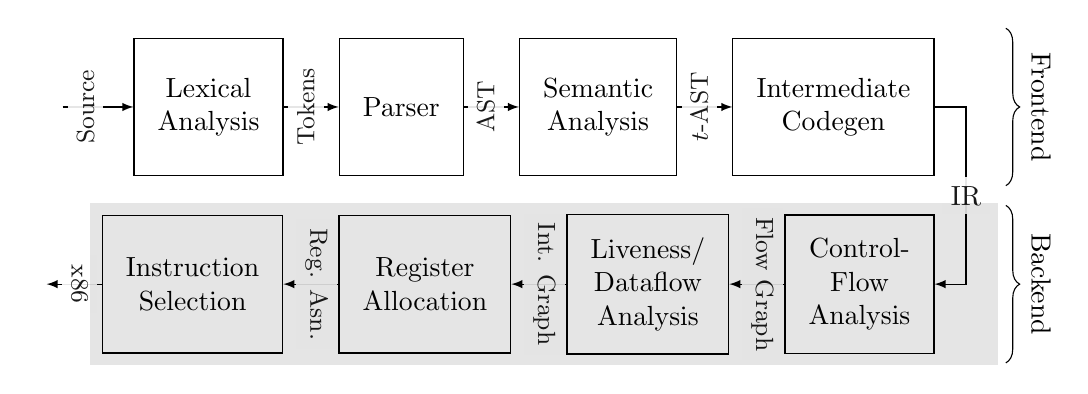
\begin{tikzpicture}


  % Nodes
  \node [box, left, align=center] (incg) at (0,2.25) {Intermediate\\Codegen};
  \node [box, left=0.7 of incg, align=center] (semant) {Semantic\\Analysis};
  \node [box, left=0.7 of semant, align=center] (parse) {Parser};
  \node [box, left=0.7 of parse, align=center] (lex) {Lexical\\Analysis};
  \node [ left=0.9 of lex, align=center] (entry) {};
  \node [box, left, align=center] (cfa) at (0,0) {Control-\\Flow\\Analysis};
  \node [box, left=0.7 of cfa, align=center] (lva)  {Liveness/\\Dataflow\\Analysis};
  \node [box, left=0.7 of lva, align=center] (alloc)  {Register\\Allocation};
  \node [box, left=0.7 of alloc, align=center] (x86)  {Instruction\\Selection};
  \node [ left=0.70 of x86, align=center] (exit) {};

  % Edge with right-angle corners
  \draw [-latex] (entry.east) -- (lex.west)  node [near start,pos=0.325,rotate=90,fill=white,opacity=0.9] {\small Source};
  \draw [-latex] (lex.east) -- (parse.west)  node [midway,pos=0.4,rotate=90,fill=white,opacity=0.9] {\small Tokens};
  \draw [-latex] (parse.east) -- (semant.west)  node [midway,pos=0.4,rotate=90,fill=white,opacity=0.9] {\small AST};
  \draw [-latex] (semant.east) -- (incg.west)  node [midway,pos=0.4,rotate=90,fill=white,opacity=0.9] {\small \(t\)-AST};
  \draw [-latex] (incg.east) -- +(0.4,0) |- node[pos=0.25,fill=white,opacity=0.9] {IR} (cfa.east);
  \draw [-latex] (cfa.west) -- (lva.east)  node [midway,pos=0.4,rotate=-90,fill=white,opacity=0.9] {\small Flow Graph};
  \draw [-latex] (lva.west) -- (alloc.east)  node [midway,pos=0.4,rotate=-90,fill=white,opacity=0.9] {\small Int. Graph};
  \draw [-latex] (alloc.west) -- (x86.east)  node [midway,pos=0.4,rotate=-90,fill=white,opacity=0.9] {\small Reg. Asn.};
  \draw [-latex] (x86.west) -- (exit.east)  node [midway,pos=0.4,rotate=-90,fill=white,opacity=0.9] {\small x86};

  % backend outline
  \fill [opacity=0.1] ([shift={(-0.15,-0.15)}]x86.south west) rectangle ([shift={(0.8,0.15)}]cfa.north east);

  \draw [decorate,decoration={brace,amplitude=5pt,mirror,raise=4ex}]
    (0.3,-1) -- (0.3,1) node[midway,xshift=3em,rotate=-90]{Backend};
  \draw [decorate,decoration={brace,amplitude=5pt,mirror,raise=4ex}]
    (0.3,1.25) -- (0.3,3.25) node[midway,xshift=3em,rotate=-90]{Frontend};
\end{tikzpicture}}
\caption{Compiler phases, backend highlighted}\label{fig:phases}
\end{figure}
\noindent Most operations of a general-purpose programming language are translated to a set of control, logic, and arithmetic instructions to be executed sequentially on a computer processor: a single circuit/chip, referred to as the \textit{central processing unit} (CPU), the design of which has varied and evolved over time.

Most CPUs are \textit{register machines}, in that they use a limited set of \textit{general-purpose registers} (GPRs) to store working values in combination with \textit{random access memory} (RAM) for mid-term, and other I/O peripherals for long-term storage. This can largely be attributed to performance, as register machines routinely outperform \textit{stack machines} \parencite{ShiYunhe2008VmsS} that are often used in VMs.
Although register machines generally also have a stack available, as being limited to mere bytes of storage is simply infeasible for most large scale applications, using it compared to GPRs is orders of magnitudes slower \cite{latency}. % FIXME: find source
Because of this, a crucial part of the backend stage for an optimizing compiler is assigning each variable  of the source program to a GPR in such a way that maximizes performance without sacrificing correctness.



The process of assigning each variable to a GPR is referred to as \textit{register allocation}, and can be approached in several different ways. This paper will seek to implement graph coloring and linear scan and evaluate them in terms of runtime performance after compilation. %% TODO: compare with time-complexity/compile-time duration?
The primary sources will be \textit{Modern Compiler Implementation in ML} \parencite{tiger} and \textit{Compilers: Principles, techniques, and tools} \parencite{dragon}, in addition to publications concerning the linear scan approach.

The implementation is written in OCaml for the most part, although there is some marginal use of Python to interact with the LLVM toolchain's debugger 'LLDB'.


%* overfladisk intro til hvad helvede register allokering er og hvorfor
    %* hovedtræk
%* rudimentær del af compilation/oversættelse fra high-level sprog til x86 er register allokering
    %* projektet er skridtet videre fra compilers kurset
    %* siger hvad jeg står ovenpå/bygger på
%snak om hvorfor jeg valgte llvm/ssa frem for x86 til global register llocation


%\section{Review of Literature}

%The two primary sources are the \textit{Modern Compiler Implementation in ML} \cite{tiger} and Dragonbook \cite{dragon}, in addition to scientific publications concerning the linear scan approach.


\section{Intermediate Representation}


Although compilers can feasibly translate from the source language to machine code of the target architecture directly, which could even be more efficient, doing so hinders the portability as machine code targeting architecture \(A\) isn't necessarily useful for targeting architecture \(B\) further down the line.

Instead of translating directly from a source language to target machine code, most compiler frontends emit IR which is intended as an abstraction over particular CPU implementations. % FIXME: er det korrekt? lol
It is by no means executable on either \(A\) or \(B\), but it is much closer to the instruction set executed on a CPU than the source language originally fed to the frontend.  This helps portability immensely, as a frontend emitting an IR no longer needs to specialize to a particular architecture, instead it can target as many as the backend supports.
Likewise, a compiler backend will support any frontend provided that they emit correct IR.

Because of this, compilation of high-level programming languages will often go no further than emitting IR, then leave the rest for a subsequent backend toolchain. This naturally leads to the LLVM toolchain, which is by far the most used compiler backend in practice. Most languages, if targeting native execution on a CPU, will have an LLVM implementation. This is true for C/C++ (Clang compiler \cite{clang}), D (LDC compiler \cite{dlang}), Swift (official Swift compiler \cite{swift}) and Rust (officilal \texttt{rustc} compiler \cite{rustc}). The use of LLVM allows for them to be compiled to completely unforeseen architectures, like web browsers with WebAssembly or even graphics cards with compute kernels \cite{backend}.

Conversely, managed languages such as Java and C\# target their own respective VMs, so they typically don't have much to gain from the LLVM toolchain. That said, some projects have attempted to implement LLVM in their translation of bytecode to native architectures,  such as LLILC which promised both \textit{just-in-time} (JIT) as well as \textit{ahead-of-time} (AOT) compilation \cite{dotnet}. Similarly, Kotlin (the spiritual successor of Java) that ordinarily targets the JVM has a native backend that compiles directly to machine code using LLVM, circumventing the need for a VM entirely \cite{kotlin}.
%Meanwhile interpreted languages like JavaScript eagerly attempt use LLVM for \textit{just-in-time} (JIT) compilation % FIXME: this is not true at all lol

%The modularization of the frontend and backend stages also helps immensely.
For example, the add function implemented in C as seen in Figure \ref{fig:addc} is compiled to the LLVM IR as seen in Figure \ref{fig:addll} after stripping optimization attributes with the \texttt{strip} utility. At this level of complexity they are largely equivalent, with the primary difference appearing to be syntactic. LLVM IR keeps the typed binary operations as well as the function construct with a return statement, although the variable names are discarded as IR is generally not for human interaction, except the function name, as this is used for linking with other object files. 

\begin{figure}[H]
   \begin{minipage}{0.48\textwidth}
     \centering
     \begin{minted}[bgcolor=LightGray]{c}
int add(int a, int b) {
  int sum = a + b;
  return sum;
}
     \end{minted}
     \caption{Arithmetic function implemented in C}\label{fig:addc}
   \end{minipage}\hfill
   \begin{minipage}{0.48\textwidth}
     \centering
     \begin{minted}[bgcolor=LightGray]{llvm}
define i32 @add (i32 %0, i32 %1) {
 %3 = add i32 %1, %0
 ret i32 %3
}
     \end{minted}
     \caption{Stripped \texttt{clang -O1 -S -emit-llvm}}\label{fig:addll}
   \end{minipage}
   \begin{center}
   \begin{minipage}{0.83\textwidth}
     \centering
     \begin{minted}[bgcolor=LightGray]{gas}
	.text
	.globl	add               # -- Begin function add
add:                                    # @add
	movl	%esi, %eax
	addl	%edi, %eax
	retq
     \end{minted}
     \caption{Output of \mintinline{bash}{clang -S} without debug markers}\label{fig:addx86}
   \end{minipage}
   \end{center}
\end{figure}
When the IR is translated to x86 as seen in Figure \ref{fig:addx86}, the virtual variables \texttt{\%0}, \texttt{\%1} and \texttt{\%2} are assigned the registers \texttt{\%esi}, \texttt{\%edi} and \texttt{\%eax} respectively. This is presumably because of several optimizations, as \texttt{\%rdi} and \texttt{\%rsi} are used to pass the first and second parameters and the \texttt{\%rax} as the return value according to the System V AMD64 ABI \cite{sysv}, so by assigning the variables to those, several \texttt{mov}s are saved. Either way, the assignment is sound and the instruction selection is reasonably close to the  source code. There are other changes as well, as marking the target section with \texttt{.text} and the \texttt{.globl} annotation to export \texttt{add} in the symbol table which permits linking with other object files, but that isn't stricly related to register allocation.


\subsection{Static Single-Assignment form}
In compiler backends, \textit{Static Single-Assignment} (SSA) form is a property that applies to some IR, including LLVM.
It is a way of representing a program such that each variable is assigned only once in
the scope of a function. Each use of the variable after definition then refers to the value  of that  single assignment, and any operations are applied by assigning the result of said operation to a freshly defined variable.

This property eliminates redefinitions entirely, making it easier to reason about data flow and in turn also speed up analysis.
It's important to note that SSA form itself doesn't inherently mandate immutability, despite only allowing for single assignment.
Rather, it provides two approaches to mutable variables: the phi nodes and load/store operations. 

Building on the earlier example, consider multiplication as  implemented in Figure \ref{fig:mulc}. Translated to LLVM IR with no optimization  can be seen in Figure \ref{fig:mulll0}, which achieves mutability by allocating a variable on the stack (lines 2-5), loading the value on use and storing on reassignment.
This means new values are loaded and assigned upon reentering a block, without reassigning the value of the source variable, which points to whatever slot was available at the time of definition.
%so any changes made at runtime by storing new values will take effect, without reassigning the source variable as it remains the address of whatever slot may be allocated on the stack.

%Although, this property also However, it's important to note that SSA form itself doesn't inherently introduce mutability;
\begin{figure}[!ht]
   \begin{minipage}{0.48\textwidth}
     \centering
     \begin{minted}[bgcolor=LightGray]{c}
extern int add(int a, int b);

int mul(int a, int b) {
  int product = 0;
  for (int i = 0; i < a; i++) {
    product = add(product, b);
  }
  return product;
}
     \end{minted}
     \caption{Multiplication function implemented in C}\label{fig:mulc}
     \vspace{2.1em}
     \begin{minted}[bgcolor=LightGray]{llvm}
declare i32 @add(i32, i32)

define i32 @mul (i32 %0, i32 %1) {
 %3 = icmp sgt i32 %0, 0
 br i1 %3, label %6, label %4
4:
 %5 = phi i32 [0, %2], [%9, %6]
 ret i32 %5
6:
 %7 = phi i32 [%10, %6], [0, %2]
 %8 = phi i32 [%9, %6], [0, %2]
 %9 = call i32 @add (i32 %8, i32 %1)
 %10 = add i32 %7, 1
 %11 = icmp eq i32 %10, %0
 br i1 %11, label %4, label %6
}
     \end{minted}
     \caption{Stripped \texttt{clang -O1 -S -emit-llvm}}\label{fig:mulll1}
   \end{minipage}\hfill
   \begin{minipage}{0.48\textwidth}
     \centering
     \begin{minted}[bgcolor=LightGray]{llvm}
define i32 @mul (i32 %0, i32 %1) {
 %3 = alloca i32
 %4 = alloca i32
 %5 = alloca i32
 %6 = alloca i32
 store i32 %0, i32* %3
 store i32 %1, i32* %4
 store i32 0, i32* %5
 store i32 0, i32* %6
 br label %7
7:
 %8 = load i32, i32* %6
 %9 = load i32, i32* %3
 %10 = icmp slt i32 %8, %9
 br i1 %10, label %11, label %18
11:
 %12 = load i32, i32* %5
 %13 = load i32, i32* %4
 %14 = call i32 @add (i32 %12, i32 %13)
 store i32 %14, i32* %5
 br label %15
15:
 %16 = load i32, i32* %6
 %17 = add i32 %16, 1
 store i32 %17, i32* %6
 br label %7
18:
 %19 = load i32, i32* %5
 ret i32 %19
}
     \end{minted}
     \caption{Stripped \texttt{clang -O0 -S -emit-llvm}}\label{fig:mulll0}
   \end{minipage}
\end{figure}
\noindent Another approach is that of Figure \ref{fig:mulll1}, which uses so-called 'phi nodes' instead.  These are a type of instruction that evaluates to a specified operand depending on which predecessor block was executed immediately prior. This circumvents the need for the same level of interior mutability as is achieved by reading/writing to memory, without violating the properties of SSA. By copying a value from the end of a predecessor to the beginning of the current block.
A Phi node represents a point in the program where the control flow merges, and it selects the appropriate version of a variable based on the path taken. This ensures that the data flow is well-defined and allows for easy analysis across different control flow paths.


%Obviously, that 
%In other words, every variable is assigned a unique version number for each assignment, and these versions are used consistently throughout the program.

\section{Control Flow Analysis}

% TODO: figure out what traces are
% TODO: mention dominators etc.


The backend of a compiler takes some form of IR as input, usually a linear sequence of instructions for each separate function. This representation is close to the level of an actual processor by design, but it isn't immediately useful for the further analysis steps needed to generate optimized code for the target architecture. %%(FIXME: why not?)
The control flow of a given program refers to the order in which instructions are executed. While the flow of most instructions is linear, in the sense that the next instruction executed is located immediately after, some transfer the flow of execution elsewhere or outright terminate it. %% FIXME: why is this important?

% mention basic block early on, they're a contiguous sequence of instructions that do not transfer control flow

A continuous flow of instructions is referred to as a \textit{basic block}, defined as a sequence of instructions with no branches in or out except for the first instruction (referred to as a \textit{leader}, immediately following either the function entry or label within it) and the last (referred to as a \textit{terminator}, as it either terminates or transfers the flow of execution). %These are often referred to as terminators and can be thought of as an entirely different categoriy of instructions. % TODO: måske drop 'can be thought of'
In order to represent the order in which instructions are executed, a \textit{control flow graph} (CFG) is introduced. It is a directed graph whose edges represent transfer of control. The type of node varies over the source material, with CFGs of the Appel text \cite{tiger} constructed over individual instructions  and the Aho text \cite{dragon} over basic blocks.
% TODO: comment on precision
Either way, leaders will have a set of predecessors and terminators a set of successors associated with them.

Terminators have one or two successors in the case of branching or none at all in the case of function exit. % These can either be associated basic blocks or individual instructions that make it up.
Unconditional branching always transfers control to the block labelled, meaning only one successor follow, whereas conditional branching could transfer to either of the two, but because control flow analysis is not concerned with data, both are considered as possible successors. % TODO: rets 

Successors of node \(n\) are denoted \( \mathit{succ}[n], \)
and while each node also has a set of predecessors associated, which consists of an  unbounded number of nodes from which control may be transferred, it isn't particularly useful in the following analysis.

%Basic blocks represent a single node in a \textit{control flow graph} (CFG), which is a directed graph whose edges denote transfer of  control flow.
%The unconditional branch terminator always transfers control flow to the block labelled, meaning only one successor will follow, whereas conditional branching could transfer to either of the two, but because control flow analysis is not concerned with data, it simply adds both as successors. % TODO: rets 


%These instructions are referred to as \textit{terminators}, as they potentially terminate a contiguous flow of execution. This subset of instructions can be further divided into \textit{branch instructions} and those concerned with handling the callstack in function/subroutine management.

%These so-called \textit{branch instructions} that alter the flow of execution are further c



% FIXME: introducer phi nodes og nævn dominators i CFA afsnittet





%hence a \textit{control flow graph} is derived from these. A terminator will branch elsewhere to continue execution. The destination of this has to be an annotated by a label, hence labels \textit{initiate} blocks.

\subsection{Building a CFG}

%\subsection{Parameterized over individual instructions}

%\subsection{Parameterized over basic blocks}


Building a graph is relatively straight forward, with the input for every function declared parsed as a tuple type named \mintinline{ocaml}{cfg}  of the form:
\begin{minted}{ocaml}
type cfg = (lbl option * block) * (lbl * block) list
\end{minted}
which consists of an optionally named entry block in the first part and a list of trailing blocks that are always named in the second. The reason for the first block to be optionally named is the fact that \textit{some} LLVM programs transfer control back to the point of entry, whereas every subsequent block needs to be named because branching can only target it by referring to its name.

From this, a CFG is constructed  using the \texttt{OCamlgraph} library \cite{ocamlgraph}, which provides several approaches with  various  structures, but the one used in this case is \texttt{Imperative.Digraph.Abstract} where the index is parameterized over \texttt{int} which corresponds to the index of the instruction starting at 0 for the first instruction to be executed. At first, a graph is constructed with the input flattened such that labels, instructions and terminators are represented as a continuous sequence as opposed to the basic blocks that is parsed from the input.

\begin{minted}[bgcolor=LightGray]{ocaml}
let flatten ((head, tail) : Ll.cfg) : insn list =
  let label l = Label l and insn i = Insn i in
  let block (b : Ll.block) = List.map insn b.insns @ [ Term b.terminator ] in
  let named_opt (n, b) = (Option.map label n |> Option.to_list) @ block b in
  let named (n, b) = Label n :: block b in
  named_opt head @ (List.map named tail |> List.flatten)
\end{minted}

\noindent This is done to simplify lookup of which graph vertex corresponds to the \(n\)th instruction/terminator. Labels, while present in the flattened list, aren't considered as they have no inherent function other than labelling the leader instruction to branch to.


%* description of blocks, how they connect etc.

%Each function defined in an LLVM program is constructed with the help of

\section{Liveness Analysis}

% * Different approaches:
%   * Naive/greedy 
%   * Dataflow analysis 
%     * forward must
%     * backwards may
%   * linear scan
%
%  TODO: comment on interrupts

Translating IR with an unbounded number of variables to a CPU with a bounded number of registers involves the process of assigning each variable a register such that no value that may be needed in the future is overwritten. %Therefore, any variable that may be used in the future is considered \textit{live}, and said to be in interference with any other variable live at any intersecting point.
Variables that are in use at a given program point are considered \textit{live}, and although variables can be assigned the same register, %if they are not in interference
variables that are live at the same time (i.e. at intersecting program points) cannot, %FIXME: why not?
in which case they are also said to be in interference with one another.
 Variables that are not in interference can be assigned the same register, and finding the precise points at which any variable is live is trivial for linear sequences of instructions. However, when conditional branching is introduced, deriving the path of execution becomes undecidable. % TODO: finish this sentence

For instance, suppose a function that calls another:

\begin{figure}[h]
\begin{minted}[linenos,bgcolor=LightGray]{llvm}
define i32 @countcall(i32 %x0) {
  %x1 = add i32 %x0, 1
  call void @printInt(i32 %x1)
  call ptr @subproc()
  ret i32 %x1
}
\end{minted}

\caption{\label{fig:undecidable}Increment, print and possibly return argument}
\end{figure}
\noindent Because of the halting problem, static analysis cannot necessarily determine if the call to \lstinline!@subproc! will return.  %which may or may not return control to the calling function:
So when assigning \lstinline!%x1! a register it is undecidable whether the variable must be live in the return instruction on line 5 in Figure \ref{fig:undecidable}.
A register must be assigned to \texttt{\%x1}, as it is used on line 3, although whether it must live across function calls can reduce the possible registers depending on the target platform and its calling conventions. % TODO: kan udvides
Because of this, any sound approach to liveness analysis will be an approximation.


In some cases it is simply impossible to assign each variable its own register without conflict along interference edges, in which case one or more variables need to be assigned to memory instead. This is also referred to as \textit{spilling} the variable/register to the stack, or the variable itself is referred to as \textit{spilled}.

 % TODO: maybe find a better exampple with a better assignment that computer can't find?
 % TODO: maybe mention exponential brute force algorithms?

A sound albeit very naive approach is to consider every variable live at every program point, such that every variable is in interference with one another, producing a fully connected interference graph.
This forces every variable to be assigned a different register, which is a viable approach for small programs with fewer variables than the set of assignable registers.
%where every variable is assigned a different register. % FIXME: find a place for: This generally isn't a very performant approach in terms of execution 
Such a heuristic is greedy in the sense that it picks an assignment known to be safe for the least amount of preprocessing possible. However, this can be a very inefficient assignment at runtime. 
When the number of variables is greater than the number of assignable registers, a variable must be spilled. A number of \(n\)  variables greater than \(k\) working registers causes \(n-k\) variables to be spilled, % TODO: skal der stå stack?
which can greatly reduce performance, but  allows for translation in linear time. %FIXME: is this even true?

\subsection{Dataflow Analysis}

% FIXME: beskriv use, def osv. sets tidligere!

Another approach, which is a more precise approximation, is a specific variant of the dataflow analysis as described in \textit{Modern Compiler Implementation in ML} \cite{tiger} and \textit{Compilers: Principles, Techniques, and Tools} \cite{dragon}. In general, dataflow analysis is the process of finding the possible paths in which data may propagate through various branches of execution.  While several applications of this exist (like constant propagation, reaching defnitions, available expressions etc.), one that is immediately beneficial in the case of liveness analysis is one that traverses a CFG in the reverse order of execution (i.e.  \textit{backwards} flow), and extracts any variable that \textit{may} be used in execution (also referred to as \textit{backwards may} analysis). % FIXME: forklar hvorfor List.rev ikke udgør backwards flow

This algorithm calculates which program points each variable may be accessed from with some conservative constraints known to maintain correctness. Specifically, these are the transfer and control-flow constraints. %, the former of which must satisfy a transfer function a
The transfer constraint is based on a \textit{transfer function} that describes how liveness is affected across instructions. For each instruction, there is a transfer function that describes how liveness changes from one point to the one immediately after. For example, as an arithmetic operation needs to be assigned a new temporary variable, the liveness of a new variable is propagated to all  instructions  executed subsequently. This is done by applying the transfer function to the current \textit{live-out} set to stop further propagation of variables defined by the currently visited instruction. % TODO: In fact, because the IR is in SSA form, the only time 
\begin{align}\label{flowin}
  \mathit{in}\left[n\right] &= \mathit{use}\left[n\right] \cup (\mathit{out}\left[n\right] - \mathit{def}\left[n\right])
\end{align}
with the \(\mathit{use}[n]\) set being defined as any variables that may be used and the \(\mathit{def}[n]\) as the set of variables defined in node \(n\). The \(\mathit{def}[n]\) either consists of one variable or equal to \(\emptyset\). The  \(\mathit{use}[n]\) set is effectively unbounded as some instructions take any \(m\) variables as parameters.

Control-flow constraints on the other hand propagate the use of variables to previously executed instructions, expecting these to be defined somewhere further up the CFG. This is done by propagating the union of the \textit{live-in} set associated with all immediate successor nodes. This is also referred to as the \textit{meet operator}, whose operator depends on the type of dataflow analysis as well, but for liveness analysis a union is performed on the \textit{live-in} sets of  any successive  nodes:
\begin{align}\label{flowout}
  \mathit{out}\left[n\right] &= \bigcup_{s\in \mathit{succ}\left[n\right]} \mathit{in}\left[s\right]
\end{align}
%in order to maintain correctness by iteratively applying a set of constraints until a fixed point is reached.
%These constraints are applied to the \(\textit{live-in}\left[i\right]\) and  \(\textit{live-out}\left[i\right]\) sets for every instruction \(i\). Both are initialized to the empty set \(\emptyset\).
%The dataflow analysis approach builds the set of variables that 
%Each type of instruction has some semantic attributes that are applied to the system state upon execution. This change is also referres to as a \textit{transfer function} as it transitions from one state to another.
%can be thought of as a \textit{transfer function} in terms of liveness, denoting which variables may be live before and after execution.
Initially, two empty sets are associated with each instruction: the \textit{live-in} and \textit{live-out} sets, which are the sets of variables that are live respectively before and after execution. Then the two equations above are applied iteratively until a fixed point is reached, i.e. an invariant point where neither \(\mathit{in}[n]\) or \(\mathit{out}[n]\) is changed for all instructions \(n\).

% TODO: onwards!


%builds sets of \textit{live-in} and  \textit{live-out} variable for each instruction.

% must be assigned in such a way that ensures its availability at every subsequent use throughout execution.

%Variables can be assigned the same register if they are not in use at the same time, so variables that are in use at the same time are said to be in interference with one another.

%Liveness analysis is the process of finding the program points at which a variable is live. This serves the function of determining which variables are live simultaneously, i.e. in conflict/interference with one another, so cannot be assigned the same physical register without overwriting the value of one another.



%Another approach that takes CFG into consideration is that of 


%These can be derived recursively by iteratively applying so-called \textit{dataflow equations} to each node in a \textit{control-flow graph} (CFG) until a stable state/fixed point is reached.

%The algorithm described in \textit{Modern Compiler Implementation in ML} \cite{tiger} and \cite{dragon} is based on the following equations for the live-in and live-out variables respectively:
%where \(use\left[n\right]\) is the set of all dependent variables, \(def\left[n\right]\) is the set of all variables defines and \(succ\left[n\right]\) is the set of all immediate successor nodes of \(n\).

%The structure of the CFG is inherently vague as both   \cite{tiger} and \textit{Compilers : Principles, Techniques, and Tools} \cite{dragon}, while based on the same underlying % TODO: fix references
%conceptions of dataflow, have different approaches to nodes of a CFG, with the former taking each individual instruction into consideration and the latter each basic block. Either of these approaches are sound 


% TODO: try int set instead of symbols

%The purpose of liveness analysis is to determine which variables are live at which program point, which in turn is used to 

%\subsubsection{Implementation}

The simplest equations to implement are the \lstinline!def! and \lstinline!use! functions, as all of the values of interest are located immediately within the instruction itself and not hidden behind some layer of indirection:
\begin{minted}[linenos,bgcolor=LightGray]{ocaml}
let def (s : S.SS.t) (insn : Cfg.insn) =
  match insn with Insn (Some dop, _) -> S.SS.add dop s | _ -> s

let use (s : S.SS.t) (insn : Cfg.insn) =
  let op o s = match o with Ll.Id i -> S.SS.add i s | _ -> s in
  let po = Fun.flip op in
  match insn with
  | Insn (_, AllocaN (_, (_, o))) (* | Bitcast _ | ... | Zext _ *) ->
      op o s
  | Insn (_, Binop (_, _, l, r)) (* | Icmp _ | Store _ *) ->
      op l s |> op r
  | Insn (_, Call (_, _, args)) -> List.map snd args |> List.fold_left po s
  | Insn (_, Gep (_, bop, ops)) -> List.fold_left po (op bop s) ops
  | Insn (_, Select (c, (_, l), (_, r))) -> op c s |> op l |> op r
  | Insn (_, PhiNode (_, ops)) -> List.map fst ops |> List.fold_left po s
  | Term (Ret (_, Some o) | Cbr (o, _, _)) -> op o s
  | _ -> s
\end{minted}
Where \lstinline!S.SS! is a \lstinline!Set.S! module built over the \lstinline!symbol! type found in \lstinline!lib/symbol.ml!:
\begin{minted}[linenos,bgcolor=LightGray]{ocaml}
type symbol = string * int
(* ... *)
module SS = Set.Make (struct
  type t = symbol
  let compare (_, n1) (_, n2) = compare n1 n2
end)
type set = SS.t
\end{minted}

\noindent The \texttt{flowin} function corresponds to the \textit{live-in} equation \eqref{flowin} and is implemented as follows:
\begin{minted}[linenos,bgcolor=LightGray]{ocaml}
let flowin (i, insn) =
  let newin = S.SS.union (use insn) (S.SS.diff out.(i) (def insn)) in
  let changed = not (S.SS.equal newin in_.(i)) in
  if changed then in_.(i) <- newin;
  changed
\end{minted}
And the \texttt{flowout} function which corresponds to the \textit{live-out} equation \eqref{flowout} implemented as follows:
\begin{minted}[linenos,bgcolor=LightGray]{ocaml}
let flowout (i, _) =
  let newout =
    let succ = Cfg.G.succ g ids.(i) in
    List.fold_left
      (fun s v -> S.SS.union s in_.(Cfg.G.V.label v))
      S.SS.empty succ
  in
  let changed = not (S.SS.equal newout out.(i)) in
  if changed then out.(i) <- newout;
  changed
\end{minted}

With the actual dataflow analysis performed recursively as follows:
\begin{figure}[H]
\begin{minted}[linenos,bgcolor=LightGray]{ocaml}
let dataflow (insns : Cfg.insn list) (ids : Cfg.G.V.t array) (g : Cfg.G.t) =
  let insns = List.mapi (fun i v -> (i, v)) insns |> List.rev in
  let in_ = Array.init (List.length insns) (fun _ -> S.SS.empty) in
  let out = Array.init (List.length insns) (fun _ -> S.SS.empty) in
  let rec dataflow () =
    let flowout = (* ... *)
    let flowin = (* ... *)
    let flow changed insn = changed || flowout insn || flowin insn in
    if List.fold_left flow false insns then dataflow () else (in_, out)
  in
  dataflow ()
\end{minted}
\caption{Overall implementation of \texttt{dataflow}\label{fig:dataflow}}
\end{figure}
\noindent One particularly noteworthy thing is reversing of the flattened list of instructions on line 2 of Figure \ref{fig:dataflow}. After enumerating each entry so that the corresponding vertex can be looked up in the \texttt{ids} array, it is reversed.
The motivation for this is the fact that the \(\mathit{out}[n]\) of node \(n\) depends on \(\mathit{in}[s]\) for all successors \(s\). Since most nodes have one successor immediately after, populating this before hands is significantly more efficient.

Consider a simple program like Figure \ref{fig:countc} that only prints integers incrementally up until \texttt{argc}, in LLVM-{}-  that would consist of one loop with one phi node as seen in Figure \ref{fig:count1ll}. The number of iterations is nearly halfed when reverseing the list of instructions prior to dataflow as can be seen on \ref{tab:countll-rev-steps} when compared to \ref{tab:countll-steps}.

\begin{figure}[H]
  \begin{minipage}[b]{0.48\textwidth}
     \centering
     \begin{minted}[linenos,bgcolor=LightGray]{c}
#include <stdio.h>

int main(int argc, char **argv) {

  for (int i = 1; i <= argc; i++) {
    printf("%d!\n", i);
  }

  return 0;
}
     \end{minted}
     \caption{\texttt{cat tests/count.ll}}\label{fig:countc}
   \end{minipage}\hfill
   \begin{minipage}[b]{0.48\textwidth}
     \centering
     \begin{minted}[linenos,bgcolor=LightGray]{llvm}
define i32 @main (i32 %0, i8* %1) {
 %3 = icmp slt i32 %0, 1
 br i1 %3, label %4, label %5
4:
 ret i32 0
5:
 %6 = phi i32 [%8, %5], [1, %2]
 %7 = call i32 (i8*, ...) @printf (i8* @.str, i32 %6)
 %8 = add i32 %6, 1
 %9 = icmp eq i32 %6, %0
 br i1 %9, label %4, label %5
}
     \end{minted}
     \caption{Stripped \texttt{clang -O1 -S -emit-llvm}}\label{fig:count1ll}
   \end{minipage}
\end{figure}



%\begin{NiceTabular}{|W{c}{0.5cm}|W{c}{0.5cm} W{c}{0.5cm}|W{c}{0.5cm} W{c}{0.5cm}|W{c}{0.5cm} W{c}{0.5cm}|W{c}{0.5cm} W{c}{0.5cm}|W{c}{0.5cm} W{c}{0.5cm}|W{c}{0.5cm} W{c}{0.5cm}|W{c}{0.5cm} W{c}{0.5cm}|W{c}{0.5cm} W{c}{0.5cm}|}


\begin{table}[H]
\makebox[\textwidth][c]{
\begin{NiceTabular}{|c|c c|c c|c c|c c|c c|c c|c c|c c|}
  \hline
  i & use & def & in & out & in & out & in & out & in & out & in & out & in & out & in & out\\
  \hline
  0  & 0  & 3 & 0  & 3 & 0  & 3,8 & 0,8  & 3,8 & 0,8  & 3,8 & 0,8  & 0,3,8 & 0,8  & 0,3,8 & 0,8  & 0,3,8\\
  1  & 3  &  & 3  & 8 & 3,8  & 8 & 3,8  & 8 & 3,8  & 0,8 & 0,3,8  & 0,8 & 0,3,8  & 0,8 & 0,3,8  & 0,8\\
  2  &   &  &   &  &   &  &   &  &   &  &   &  &   &  &   & \\
  3  &   &  &   &  &   &  &   &  &   &  &   &  &   &  &   & \\
  4  &   &  &   & 8 & 8  & 8 & 8  & 8 & 8  & 0,8 & 0,8  & 0,8 & 0,8  & 0,8 & 0,8  & 0,8\\
  5  & 8  & 6 & 8  & 6 & 8  & 6 & 8  & 0,6 & 0,8  & 0,6 & 0,8  & 0,6 & 0,8  & 0,6 & 0,8  & 0,6\\
  6  & 6  & 7 & 6  & 6 & 6  & 0,6 & 0,6  & 0,6 & 0,6  & 0,6 & 0,6  & 0,6 & 0,6  & 0,6 & 0,6  & 0,6\\
  7  & 6  & 8 & 6  & 0,6 & 0,6  & 0,6 & 0,6  & 0,6 & 0,6  & 0,6,8 & 0,6  & 0,6,8 & 0,6  & 0,6,8 & 0,6  & 0,6,8\\
  8  & 0,6  & 9 & 0,6  & 9 & 0,6  & 9 & 0,6  & 8,9 & 0,6,8  & 8,9 & 0,6,8  & 8,9 & 0,6,8  & 0,8,9 & 0,6,8  & 0,8,9\\
  9  & 9  &  & 9  &  & 9  & 8 & 8,9  & 8 & 8,9  & 8 & 8,9  & 0,8 & 0,8,9  & 0,8 & 0,8,9  & 0,8\\
  \hline
\end{NiceTabular}
}
\caption{Output of \texttt{dune exec build -{}- -t lva -v tests/count1.ll}}
\label{tab:countll-rev-steps}
\end{table}

\begin{table}[H]
\makebox[\textwidth][c]{
\setlength{\tabcolsep}{0.9pt}
\begin{NiceTabular}{|c|c c|c c|c c|c c|c c|c c|c c|c c|c c|c c|c c|c c|}
  \hline
  i & use & def & in & out & in & out & in & out & in & out & in & out & in & out & in & out & in & out & in & out & in & out & in & out\\
  \hline
  0  & 0  & 3 & 0  &  & 0  & 3 & 0  & 3 & 0  & 3,8 & 0,8  & 3,8 & 0,8  & 3,8 & 0,8  & 3,8 & 0,8  & 3,8 & 0,8  & 3,8 & 0,8  & 0,3,8 & 0,8  & 0,3,8\\
  1  & 3  &  & 3  &  & 3  & 8 & 3,8  & 8 & 3,8  & 8 & 3,8  & 8 & 3,8  & 8 & 3,8  & 8 & 3,8  & 0,8 & 0,3,8  & 0,8 & 0,3,8  & 0,8 & 0,3,8  & 0,8\\
  2  &   &  &   &  &   &  &   &  &   &  &   &  &   &  &   &  &   &  &   &  &   &  &   & \\
  3  &   &  &   &  &   &  &   &  &   &  &   &  &   &  &   &  &   &  &   &  &   &  &   & \\
  4  &   &  &   &  &   & 8 & 8  & 8 & 8  & 8 & 8  & 8 & 8  & 8 & 8  & 8 & 8  & 0,8 & 0,8  & 0,8 & 0,8  & 0,8 & 0,8  & 0,8\\
  5  & 8  & 6 & 8  &  & 8  & 6 & 8  & 6 & 8  & 6 & 8  & 6 & 8  & 0,6 & 0,8  & 0,6 & 0,8  & 0,6 & 0,8  & 0,6 & 0,8  & 0,6 & 0,8  & 0,6\\
  6  & 6  & 7 & 6  &  & 6  & 6 & 6  & 6 & 6  & 0,6 & 0,6  & 0,6 & 0,6  & 0,6 & 0,6  & 0,6 & 0,6  & 0,6 & 0,6  & 0,6 & 0,6  & 0,6 & 0,6  & 0,6\\
  7  & 6  & 8 & 6  &  & 6  & 0,6 & 0,6  & 0,6 & 0,6  & 0,6 & 0,6  & 0,6,8 & 0,6  & 0,6,8 & 0,6  & 0,6,8 & 0,6  & 0,6,8 & 0,6  & 0,6,8 & 0,6  & 0,6,8 & 0,6  & 0,6,8\\
  8  & 0,6  & 9 & 0,6  &  & 0,6  & 9 & 0,6  & 8,9 & 0,6,8  & 8,9 & 0,6,8  & 8,9 & 0,6,8  & 8,9 & 0,6,8  & 8,9 & 0,6,8  & 8,9 & 0,6,8  & 0,8,9 & 0,6,8  & 0,8,9 & 0,6,8  & 0,8,9\\
  9  & 9  &  & 9  & 8 & 8,9  & 8 & 8,9  & 8 & 8,9  & 8 & 8,9  & 8 & 8,9  & 8 & 8,9  & 0,8 & 0,8,9  & 0,8 & 0,8,9  & 0,8 & 0,8,9  & 0,8 & 0,8,9  & 0,8\\
  \hline
\end{NiceTabular}
}
\caption{Output of \texttt{dune exec build -{}- -t lva -v -r tests/count1.ll}}
\label{tab:countll-steps}
\end{table}

\noindent This is unnoticeable for snippets of marginal size like most examples included, but when applied to functions with a significant amount of def-use paths, it can be quite consequential. For \texttt{tests/sha256.ll} for instance, the running time of this analysis is effectively doubled:

\begin{minted}{bash}
$ time dune exec build -- tests/sha256.ll  -t lva -r
33,69s user 0,04s system 99% cpu 33,765 total
$ time dune exec build -- tests/sha256.ll  -t lva
17,26s user 0,05s system 99% cpu 17,335 total
\end{minted}


\subsection{Interference Graph}

The purpose of conducting dataflow analysis as above is finding variables that may be assigned the same register. This is done by building an interference graph, which is an undirected graph, whose nodes represent variables and edges that signify interference between them, i.e. variables \(a\) and \(b\) live at intersecting program points is represented with an edge \((a,b)\).


Constructing an interference graph only depends on the \textit{live-out} set and type of instruction. If the instruction defines a variable, said variable is in interference with all variables in the \textit{live-out} set. There is one exception however: according to the Appel text, move instructions (i.e. phi nodes in the case of SSA form) are given special consideration. The purpose of phi nodes is to copy/move a certain value from a certain predecessor, so they are not necessarily in conflict for being live at the same time. Rather it would often benefit if they were assigned the same register to spare unnecessary moves. % TODO: uddyb hvorfor de ikke er i interference?


Because of this, for any phi node of the form 
\begin{equation}
  a = \Phi (b_1, ..., b_n) \label{phi}
\end{equation}
add edges to all \textit{live-out} variables not in \(\{b_1, ..., b_n\}\)
\[
  \forall b_j \in \mathit{out}[i] \setminus \{b_1, ..., b_n\}, \text{add\_edge}(a, b_j),
\]
and for any other instruction that defines a variable \(a\)
\[
  \forall b_j \in \{b_1, ..., b_n\}, \text{add\_edge}(a, b_j).
\]
Although the Appel text \cite{tiger} describes interference of variables with concrete registers as well as overlapping variables, this isn't considered in this implementation % FIXME: why??
for simplicity's sake.

Again the \texttt{OCamlgraph} library is used, but this time \texttt{Imperative.Graph.Abstract} is parameterized over the aforementioned set type \texttt{S.SS.t}. % FIXME: whyyy????


\begin{figure}[H]
\begin{minted}[linenos,bgcolor=LightGray]{ocaml}
let interf (params : Ll.uid list) (insns : Cfg.insn list) _ (out : S.SS.t array)
    : G.V.t S.table * G.t =
  let g = G.create () in
  let vert e t = (* .. *) in
  let vert2 t e = vert e t |> snd and vert3 e t = vert e t |> snd in
  (* add params *)
  let t = List.fold_left vert2 S.ST.empty params in
  (* connect all params *)
  let edge v1 v2 t = (* .. *) in
  let param t p1 =
    let param t p2 = if p1 <> p2 then edge p1 p2 t else t in
    List.fold_left param t params
  in
  let t = List.fold_left param t params in
  (* add all defs *)
  let setverts t s = S.SS.fold vert3 s t in
  let t = List.map (def S.SS.empty) insns |> List.fold_left setverts t in
  let defoutedges t (i, n) =
    let defs = def S.SS.empty n in
    let outedge e1 t = S.SS.fold (edge e1) out.(i) t in
    S.SS.fold outedge defs t
  in
  let t = List.mapi (fun i n -> (i, n)) insns |> List.fold_left defoutedges t in
  (t, g)
\end{minted}
\caption{Overall implementation of \texttt{interf}\label{fig:interf}}
\end{figure}

\noindent For instance, the LLVM-{}- program of Figure \ref{fig:countdown.ll}, a simple handwritten program that counts down from \texttt{\%argc}, would translate the interference graph of Figure \ref{fig:countdown.dot}. % TODO: explain step wise?

\begin{figure}[H]
     \centering
     \begin{minipage}[b]{0.57\textwidth}
     \begin{minted}[bgcolor=LightGray]{llvm}
define i32 @main (i32 %argc, i8** %argv) {
entry:
 br label %loop
loop:
 %c1 = phi i32 [%argc, %entry], [%c2, %loop]
 call void @printf (i8* @fmt, i32 %c1)
 %c2 = sub i32 %c1, 1
 %cn = icmp sgt i32 %c2, 0
 br i1 %cn, label %loop, label %exit
exit:
 ret i32 0
}
     \end{minted}
     \caption{\texttt{cat tests/countdown.ll}}\label{fig:countdown.ll}
   \end{minipage}
   \begin{minipage}[b]{0.42\textwidth}
     \centering
     \includesvg[height=15em]{countdown.simple}
     \caption{\texttt{dune exec build -- -t dot}}\label{fig:countdown.dot}
   \end{minipage}
\end{figure}

%module G = Imperative.Graph.Abstract (struct
  %type t = S.SS.t
%end)



%\section{CFG -> INTERF}

%* describe the dataflow algorithm from the book
%* describe the interference criteria from the book

%\section{INTERF -> DOT}

%* ez ???

%\section{INTERF -> DOT/Assignment}

%* list of methods for coalescing/allocating:
%   * ocamlgraph builtin
%   * greedy 
%   * briggs
%   * george
%   * welsh-powell?
\section{Graph Coloring}
Once an interference graph is constructed, the actual assignments can be found using graph coloring.
Graph coloring is a problem in graph theory where the goal is to assign colors to the vertices of a graph in such a way that no adjacent vertices are assigned the same color.
A graph that can be colored using \(k\) different colors is referred to as \(k\)-colorable and the minimum number of colors needed to be assigned is also called its' chromatic number.
Although this problem is known to be NP-complete  \cites[229]{tiger}[510]{dragon}, the heuristic as introduced in
both the Appel \cite[229]{tiger}, and Aho et al. \cites[557]{dragon} texts,
is a linear time approximation to this problem is described below.

\subsection{Coloring by simplification}

The \textit{simplification} algorithm, also known as Chaitin's algorithm \cite{chaitin}, 
 is an iterative approach wherein nodes known to be colorable are removed and pushed to a stack until either an empty graph remains, in which case the original graph is \(k\)-colorable,  or nodes with more than \(k\) neighbours remain.
In this case a node is chosen to be spilled after which the process is started over. This is repeated until every node has been removed successfully, after which the vertices are assigned by popping them from the stack. Each of these are known to be \(k\)-colorable because of the earlier criteria of having less than \(k\) neighbors.

%Let \(k\) be the number of working registers available on the target architecture. After building the interference graph \(G\), a node \(n\) with fewer than \(k\) neighbors is chosen. As \(n\) has at most \(k-1\) neighbors, it can be removed safely, effectively simplifying \(G\). It is pushed to a stack to preserve the order in which they are removed so that \(G\) can be rebuilt and the corresponding registers can be assigned correctly once a \(k\)-colorable assignment is found.


To perform the simplication algorithm on the previous example of Figure \ref{fig:countdown.ll}, its interference graph seen on Figure \ref{fig:countdown.dot} only has one node of degree 4 with the ones remaining all being \(\leq 2\). This wouldn't be a problem on modern day processors most of which have \textasciitilde 16 or so GPRs, but for the sake of clearness one can imagine a register machine of \(k=2\) working registers.

If at first a single node of insignificant degree (i.e. \(< 2\)) is selected, it is then removed and pushed to a stack. In Figure \ref{fig:countdown.dot} only \texttt{\%argv} and \texttt{\%c1} are of insignificant degree, so either of those is chosen to be removed (represented with dashed borders and edges) as can be seen on Figure \ref{fig:countdown.dot2} and \ref{fig:countdown.dot3} and pushed to the stack of variables to be colored as can be seen on Figure \ref{fig:countdown.stack2} and \ref{fig:countdown.stack3}.




% Side by side figures 
\begin{figure}[H]
  \centering
  \begin{minipage}[b]{0.31\linewidth}
    \begin{subfigure}[b]{0.70\textwidth}
      \includesvg[height=10em]{countdown.simple2}
      \caption{Graph}\label{fig:countdown.dot2}
    \end{subfigure}
    \begin{subfigure}[b]{0.27\textwidth}
      \centering
        \texttt{\%c1}
        \vspace{0.5em}
      \caption{Stack}\label{fig:countdown.stack2}
    \end{subfigure}
    \caption{Push \texttt{\%c1}}
  \end{minipage}%
  \begin{minipage}[b]{0.31\linewidth}
    \begin{subfigure}[b]{0.70\textwidth}
      \includesvg[height=10em]{countdown.simple3}
      \caption{Graph}\label{fig:countdown.dot3}
    \end{subfigure}
    \begin{subfigure}[b]{0.27\textwidth}
      \centering
        \texttt{\%argv}\\
        \texttt{\%c1}
        \vspace{0.5em}
      \caption{Stack}\label{fig:countdown.stack3}
    \end{subfigure}
    \caption{Push \texttt{\%argv}}
  \end{minipage}%
  \begin{minipage}[b]{0.31\linewidth}
    \begin{subfigure}[b]{0.70\textwidth}
      \includesvg[height=6em]{countdown.simple4}
      \caption{Graph}\label{fig:countdown.dot4}
    \end{subfigure}
    \begin{subfigure}[b]{0.27\textwidth}
      \caption{Stack}\label{fig:countdown.stack4}
    \end{subfigure}
    \caption{Spill \texttt{\%c2}}
  \end{minipage}%
\end{figure}
\noindent From this point onwards  nothing can be done to further simplify the graph as all of the remaining nodes are of significant degree (\(\geq 2\)). Therefore, one of the remaining nodes is spilled to memory and entirely removed from the graph as can be seen on Figure \ref{fig:countdown.dot4} and the stack reset as can be seen on Figure \ref{fig:countdown.stack4}.

\begin{figure}[H]
  \centering
  \begin{minipage}[c]{0.32\linewidth}
    \begin{subfigure}[b]{0.70\textwidth}
      \includesvg[height=6em]{countdown.simple5} 
      \caption{Graph}\label{fig:countdown.dot5}
    \end{subfigure}
    \begin{subfigure}[b]{0.27\textwidth}
      \centering
        \texttt{\%cn}
        \vspace{0.5em}
      \caption{Stack}\label{fig:countdown.stack5}
    \end{subfigure}
    \caption{Push \texttt{\%cn}}
  \end{minipage}%
  \begin{minipage}[c]{0.32\linewidth}
    \begin{subfigure}[b]{0.70\textwidth}
      \includesvg[height=6em]{countdown.simple6} 
      \caption{Graph}\label{fig:countdown.dot6}
    \end{subfigure}
    \begin{subfigure}[b]{0.27\textwidth}
      \centering
        \texttt{\%argv}\\
        \texttt{\%cn}
        \vspace{0.5em}
      \caption{Stack}\label{fig:countdown.stack6}
    \end{subfigure}
    \caption{Push \texttt{\%argv}}
  \end{minipage}%
  \begin{minipage}[c]{0.32\linewidth}
    \begin{subfigure}[b]{0.70\textwidth}
      \includesvg[height=6em]{countdown.simple7} 
      \caption{Graph}\label{fig:countdown.dot7}
    \end{subfigure}
    \begin{subfigure}[b]{0.27\textwidth}
      \centering
      \texttt{\%argc}\\
      \texttt{\%argv}\\
      \texttt{\%cn}
      \vspace{0.5em}
      \caption{Stack}\label{fig:countdown.stack7}
    \end{subfigure}
    \caption{Push \texttt{\%argc}}
  \end{minipage}%
\end{figure}

\noindent After spilling \texttt{\%c2}, the process is repeated. First by pushing \texttt{\%cn} (Figure \ref{fig:countdown.dot5} and \ref{fig:countdown.stack5}), then \texttt{\%argv} (Figure \ref{fig:countdown.dot6} and \ref{fig:countdown.stack6}) and finally \texttt{\%argc} (Figure \ref{fig:countdown.dot7} and \ref{fig:countdown.stack7}). One thing of note is the fact that the order in which this is happening is irrelevant, so long as variables pushed are of insignificant degree. For instance, \texttt{\%argc} was of degree 3 in Figure \ref{fig:countdown.dot4}, but as more and more of its neighbors are pushed it's degree decreases to a point where only \texttt{\%argc} and \texttt{\%c1} are yet to be pushed to the stack.


\begin{figure}[H]
  \centering
  \begin{minipage}[c]{0.32\linewidth}
    \begin{subfigure}[b]{0.70\textwidth}
      \includesvg[height=6em]{countdown.simple8} 
      \caption{Graph}\label{fig:countdown.dot8}
    \end{subfigure}
    \begin{subfigure}[b]{0.27\textwidth}
      \centering
      \texttt{\%c1}\\
      \texttt{\%argc}\\
      \texttt{\%argv}\\
      \texttt{\%cn}
      \vspace{0.5em}
      \caption{Stack}\label{fig:countdown.stack8}
    \end{subfigure}
    \caption{Push \texttt{\%c1}}\label{fig:countdown8}
  \end{minipage}%
  \begin{minipage}[c]{0.32\linewidth}
    \begin{subfigure}[b]{0.70\textwidth}
      \includesvg[height=6em]{countdown.simple9} 
      \caption{Graph}\label{fig:countdown.dot9}
    \end{subfigure}
    \begin{subfigure}[b]{0.27\textwidth}
      \centering
      \texttt{\%argc}\\
      \texttt{\%argv}\\
      \texttt{\%cn}
      \vspace{0.5em}
      \caption{Stack}\label{fig:countdown.stack9}
    \end{subfigure}
    \caption{Pop \texttt{\%c1}}\label{fig:countdown9}
  \end{minipage}%
  \begin{minipage}[c]{0.32\linewidth}
    \begin{subfigure}[b]{0.70\textwidth}
      \includesvg[height=6em]{countdown.simple10} 
      \caption{Graph}\label{fig:countdown.dot10}
    \end{subfigure}
    \begin{subfigure}[b]{0.27\textwidth}
      \centering
      \texttt{\%argv}\\
      \texttt{\%cn}
      \vspace{0.5em}
      \caption{Stack}\label{fig:countdown.stack10}
    \end{subfigure}
    \caption{Pop \texttt{\%argc}}
  \end{minipage}%
\end{figure}

\noindent As the last variable \texttt{\%c1} is pushed in Figure \ref{fig:countdown8} and an empty graph remains, the process of reconstructing the graph can begin. When popping \texttt{\%c1} in Figure \ref{fig:countdown9}, it can be assigned any of the two colors as it has no neigbors adjacent, so either is chosen. On the other hand, when assigning \texttt{\%argc}, it's only adjacent naighbor \texttt{\%c1} is already assigned red so only blue remains. Likewise, for \texttt{\%argv} and \texttt{\%cn} their only immediately adjacent neighbor of \texttt{\%argc} causes them to be assigned red as can be seen on Figure \ref{fig:countdown11} and \ref{fig:countdown12}.

\begin{figure}[H]
  \centering
  \begin{minipage}[c]{0.32\linewidth}
    \begin{subfigure}[b]{0.70\textwidth}
      \includesvg[height=6em]{countdown.simple11} 
      \caption{Graph}\label{fig:countdown.dot11}
    \end{subfigure}
    \begin{subfigure}[b]{0.27\textwidth}
      \centering
      \texttt{\%cn}
      \vspace{0.5em}
      \caption{Stack}\label{fig:countdown.stack11}
    \end{subfigure}
    \caption{Pop \texttt{\%argv}} \label{fig:countdown11}
  \end{minipage}%
  \begin{minipage}[c]{0.32\linewidth}
    \begin{subfigure}[b]{0.70\textwidth}
      \includesvg[height=6em]{countdown.simple12} 
      \caption{Graph}\label{fig:countdown.dot12}
    \end{subfigure}
    \begin{subfigure}[b]{0.27\textwidth}
      \caption{Stack}\label{fig:countdown.stack12} 
    \end{subfigure}
    \caption{Pop \texttt{\%c1}}\label{fig:countdown12} 
  \end{minipage}%
\end{figure}
\noindent The final coloring of Figure \ref{fig:countdown12} leads to the assignment 
\begin{align*}
  \mathit{assign[\texttt{\%argv}]} = \mathit{assign[\texttt{\%c1}]} = \mathit{assign[\texttt{\%cn}]} &= \texttt{\%red}\\
  \mathit{assign[\texttt{\%argc}]} &= \texttt{\%blue}
\end{align*}
and the spilled variable \texttt{\%c2}
\[
  \mathit{assign[\texttt{\%c2}]} = \texttt{stackslot(0)}
\]


%  (i.e. \(\mathit{deg}(n) < k\))

%It must hold that \(G-\{n\}\) is \(k\)-colorable if \(G\) is \(k\)-colorable 


%% TODO
%* optimistic coloring
\subsection{Coalescing}


Coalescing is the process of eliminating moves/copies of data from one GPR to another by combining their interference graph nodes.  This is similar to but  not the same as  the lack of interference edges between variables that are subject to move operations. This is because variables \(a\) and \(b\) may still be assigned different registers or even spilled if,  for instance, either of them are of significant degree. Coalescing joins nodes \(a\) and \(b\) to node \(ab\) preserving the edges of both to maintain soundness.

Since all edges are preserved, the resulting node \(ab\) may be of a much higher degree. Because of this, only strategies that produce a \(k\)-colorable graph are worth considering, as additional spills negate the purpose entirely. One of the  strategies introduced in the Appel text is the \textit{Briggs} strategy  \cite[232]{tiger}, in which nodes \(a\) and \(b\) can be coalesced if and only if the resulting node \(ab\) is of insignificant degree  (i.e. \(\leq K\)).

Since the only move operations in use in LLVM-{}- are phi nodes, only variables that are subject to this sort of operation are eligible to be coalesced in this form. 
Variables that may be coalesced can be thought of as having a different sort of edge, quite the opposite of interference edges, in fact they can be thought of as a sort of 'preference edge'.
Strictly speaking, one could optimize many more mov instructions away if 



\section{Linear Scan}
Another approach that does not depend on liveness analysis i the linear scan algorithm.
It is a simple and efficient approach that performs a linear pass over IR to produce a register assignment significantly faster than all of the steps involved with graph coloring.

The primary text is \textit{Linear Scan Register Allocation} \cite{linear}, the execution of which also relies on prior liveness analysis.


% TODO: find ud af hvad binpacking er
%
%Write about Appel book.

%Write about SSA form liveness analysis. 

%Keywords: program points, dataflow equations, fixed point


% TODO: find ud af om man skal henvise til kurser på au på speciel form

%* todo: ssa/llvm vs appel analysis
%* henvis til blog posts som archive
%    * så tæller det som litteratur
%* tag essensen ud af hvad der bliver sagt i teksten
    %* som er relevant for mit arbejde
%
%* HENVIS TIL KAPITEL 19 OM SSA FORM
%
%* linear scan approach
%
%* snak om hvilke dele af bogen i hvilken rækkefølge
%
%Appel (208p):
%*   Translation To Intermediate Code (153-179, 26p)
%*   Basic Blocks And Traces (179-193, 14p)
%*   Instruction Selection (193-219, 26p)
%*   Liveness Analysis (219-237, 18p)
%*   Register Allocation (237-267, 30p)
%*   Dataflow Analysis (387-415, 28p)
%*   Loop Optimizations (415-439, 24p)
%*   Static Single Assignment Form (439-481, 42p)
%
%*using IR when only translating from one language to another:
%
%>Even when only one front end and one back end are being built, a good IR can modularize the task, so that the front end is not complicated with machine-specific details, and the back end is not bothered with information specific to one source language.

%TODO: As linear scan 

%Live ranges for each of the temporaries are derived by visiting each instruction of each control flow block and examining its \textit{uses} and \textit{defs}.

\section{Instruction Selection}

%% NOTE: special implementations
%%
%% * phi nodes
%% * calling convention:
%%   * save/restore callee saved registers in pro/epilogue
%%   * save/restore caller saved registersk before call
%% * jump flags for comparison


\subsection{LLVM-{}- instruction set}

%The intermediate representation emitted by the frontend of a compiler serves as a stepping stone independent of the target architecture. The \lstinline!LLVM! infrastructure is the industry standard in terms of bridging this gap and was consequently the library used to translate the semantically annotated abstract syntax tree to executable machine code in the 2022 compilers course. As this project is an expansion on this, it follows naturally to build on this. 

The instruction set used in this paper will be a union of the sets used in the 2022 and 2023 compilers courses in order to work as a drop-in replacement of LLVM for either of the two respective source languages:  Tiger and Dolphin. This instruction set is a subset of the one used in practice, as, for instance, neither of the languages implemented support exception handling, floating point operations and so on, and instead only strive to cover the basics of compilers.

The instructions included are
\lstinline!trunc! has only been added in order to help cover more generated LLVM. % FIXME
%with only four distinct block terminators 
%\begin{enumerate}
%    \item Unconditional \lstinline!br! followed by the label to branch to
%    \item Conditional \lstinline!br!  followed by an \lstinline!i1! condition and two labels
%    \item \lstinline!ret! followed by an optional return value
%    \item \lstinline!unreachable!
%\end{enumerate}
The branching for most of these is trivial: after successful execution the flow of all but \lstinline!br!, \lstinline!ret! and \lstinline!unreachable! will unconditionally attempt to execute the next instruction in memory (i.e. increment the instruction pointer by instruction length).

%Because of this, these instructions are referred to as \textit{terminators}, as their purpose is to disrupt what had otherwise been a linear flow from the beginning of this continus sequence of instructions, henceforth referred to as a \textit{basic block}.

\label{appendix:llvmis}
\begin{enumerate}
    \item binary operations \lstinline!add!, \lstinline!and!, \lstinline!ashr!, \lstinline!lshr!, \lstinline!mul!, \lstinline!or!, \lstinline!sdiv!,\\\lstinline!srem!, \lstinline!shl!, \lstinline!sub! and \lstinline!xor!
    \item integer comparison \lstinline!icmp! (conditions being \lstinline!eq!, \lstinline!ne!, \lstinline!sge!, \lstinline!sgt!, \lstinline!sle! and \lstinline!slt!)
    \item memory/address operations \lstinline!alloca!, \lstinline!gep!, \lstinline!load! and \lstinline!store!
    \item  \lstinline!mov! operations \lstinline!gep!, \lstinline!phi!, \lstinline!ptrtoint!, \lstinline!trunc!, and \lstinline!zext!
    \item control flow operations \lstinline!br!, \lstinline!call! and \lstinline!ret!
    \item a  nullary block terminator \lstinline!unreachable!
\end{enumerate}

%%%
\subsection{Translating LLVM-{}- to x86}

Translating each IR instruction to x86 correctly is a matter of eliminating unintended side-effects. Each LLVM-{}- instruction is defined to have only one purpose, %% FIXME is purpose the right word?
as concepts such as calling conventions, stack frames, or a \lstinline!FLAGS! register are completely abstracted over in order to remain platform independent.

In contrast, the x86 \textit{instruction set architecture} (ISA) is targeting a  \textit{complex instruction set computer} (CISC) family of processors, the instructions of which perform a much broader set of operations \cite[p.~190]{tiger}. This is is in part due to pipelining, i.e. an abstraction over the concrete implementation of the actual processor, which in turn is made for the sake of performance.

An example of this would be the division/remainder operation: since integer division is a non-trivial iterative process wherein both the quotient and remainder is needed throughout, the result of both of these is stored in the \lstinline!%rax! and \lstinline!%rdx! registers respectively. This means two operations are performed simultaneously regardless of which value is used, hence they need to be restored before executing the next instruction, as any variables assigned to \lstinline!%rax! or \lstinline!%rdx! will be overwritten.

\begin{center}
\begin{tabular}{|c||c|c|c|c|} 
 \hline
 add & addx & \{\}\\
 \hline
 mul & imul & \{ \%rax \} \\
 \hline
 sdiv & idivx & \{\%rax, \%rdx\} \\
 \hline
 srem & idivx & \{\%rax, \%rdx \\
 \hline
   call & callx & \{\%rax, \textit{caller saved registers}\} \\
 \hline
 \hline
\end{tabular}
\end{center}


\subsubsection{Implementing \mintinline{llvm}{call} instructions}

The \mintinline{llvm}{call} operation is by far the most complicated one. Mostly because of calling conventions,
The \mintinline{gas}{%rax} register is zeroed before 

\subsubsection{Implementing \mintinline{llvm}{phi} instructions}
Another irregular instruction is the \mintinline{llvm}{phi} instruction representing the \(\Phi\)-functions. Their  intended purpose is to copy data from whichever predecessor node was executed.
%, so intuitively, additional branching must be incurred to select the correct value to merge, but this isn't the case. Rather, 
As opposed to the other instructions that are only concerned with transferring the current state to another, this operation needs to concern itself with what was executed immediately prior.
Fortunately there is no need to further complicate the scenario with additional state for the past executed block, as simply moving from \(\mathit{assign}[b_i]\) to \(\mathit{assign}[a]\) immediately prior to branching into the block whose header contains a phi node of the form \eqref{phi} will suffice.

\begin{figure}[H]
   \begin{minipage}{0.48\textwidth}
     \centering
     \begin{minted}[linenos,bgcolor=LightGray]{llvm}
define i32 @main (i32 %0) {
1:
 %2 = icmp sgt i32 %0, 0
 br i1 %2, label %3, label %9
3:
 %4 = phi i32 [%0, %1], [%7, %3]
 %5 = phi i32 [0, %1], [%6, %3]
 %6 = add i32 %5, %0
 %7 = sub i32 %4, 1
 %8 = icmp ugt i32 %7, 0
 br i1 %8, label %3, label %9
9:
 %10 = phi i32 [0, %1], [%6, %3]
 ret i32 %10
}
     \end{minted}
     \caption{\texttt{cat tests/square0.ll}}\label{fig:square0ll}
   \end{minipage}\hfill
   \begin{minipage}{0.48\textwidth}
     \centering
     \begin{minted}[linenos,bgcolor=LightGray]{gas}
_main$3:
  # ...
  # br i1 %8, label %3, label %9
  movq %rdx, %rax
  cmpq $0, %rax
  movq %rbx, %rax
  movq %rax, %rdx
  je _main$9
  movq %rsi, %rax
  movq %rax, %rsi
  movq %rbx, %rax
  movq %rax, %rdx
  jmp _main$3
_main$9:
  # ...
     \end{minted}
     \caption{\texttt{dune exec build -{}- -t x86}}\label{fig:square0s}
   \end{minipage}
\end{figure}

\noindent Notice for instance Figure \ref{fig:square0ll} which has three phi nodes: two in  block 3 and one in block 9, i.e. \texttt{\%0} needs to be copied to \texttt{\%4} when control is transferred from block 1 and \texttt{\%7} when transferred from block 3. Likewise the immediate value \texttt{\$0} must be copied to \texttt{\%5} when transferred from block 1 and \texttt{\%6} when transferred from block 3.
All of the relevant translation can be seen in the fragment on Figure \ref{fig:square0s}. After the comparison operation on lines 4-6 that check if the boolean condition of \texttt{\%2} is nonzero and setting \texttt{FLAGS} register accordingly, \texttt{\$0} is moved into
\(\mathit{assign}[\texttt{\%1}]\) in preparation
of transferring to \texttt{\_main\$9} if the zero flag indeed is set. If not, execution is continued in which case both \(\mathit{assign}[\texttt{\%6}]\) and \(\mathit{assign}[\texttt{\%7}]\) are moved into \(\mathit{assign}[\texttt{\%4}]\) and \(\mathit{assign}[\texttt{\%5}]\) respectively, in preperation for continuing execution at \texttt{\_main\$3}.

As \texttt{mov} operations do not change the \texttt{FLAGS} register \cite{x86asm}, having \texttt{mov} instructions between the branching instructions of \texttt{je} and \texttt{jmp} do not affect the branching. Likewise, because of the \(\mathit{use}[n]\) semantics of \(\Phi\)-functions, all \(b_i\) are in interference in one another, so may not be overwritten by the \texttt{mov}s inserted.

% FIXME: check if above is sound


%and concerning with which node was executed immediately before, this can be achieved by approaching the problem differently.

%* safest possible x86 translation
%
    %* moving sys-v abi arguments to assigned registers is treacherous

\subsection{Assessing Correctness}
It is difficult to assert the correctness of a compiler. While writing simple unit tests is easy, guaranteeing the correctness of code generated for any given input is on a different order of magnitude in terms of complexity.

Validating the correctness of each instruction translation is a complicated task given how low-level it is. One approach is attaching a debugger and examining the state before and after the translated sequence of x86 instructions is executed. The result of applying a binary operation,  for instance, should only affect the assigned register.

% TODO: kommenter på stripper

\subsubsection{Debugger Harness}
A more elaborate way of testing correctness of translation is to assert that there are no effects except for those intended. One way of achieving this is to check if a group of x86 instructions representing a single LLVM-{}- operation change any values except those expected. An approach to this is to attach a debugger, insert a breakpoint before every LLVM-{}- instruction, and ensure that only the intended registers are altered.

To achieve this, only a few changes need to be made to the codebase. A debug flag is introduced, which inserts a label before every instruction by adding a \lstinline!Breakpoint! variant of the \lstinline!ins! type before the assembly emitted of that specific operation. A unique identifier as well as a list of changes expected to be made is encoded. 
This includes a bitmask of GPRs that can possibly be changed (aside from the scratch registers of course) as well as which parts of the stack may be modified. % TODO: implement the stack checker
In addition to this, each of the labels are output with a \lstinline!.globl! directive in the file header. A file is built with these extra symbols using the \lstinline!-d! flag.

To validate that this works as intended, 


%\section{Further Optimization}

% TODO: quote computability theory infinitely many optimizations


\section{Evaluation}

While there are many approaches to assessing the quality of translation, one of the primary means is to simply measure the time taken to execute the code generated. 
Assuming the translation is sound given the previous steps taken to validate correctness in translating LLVM-{}- to x86, it is a solid foundation for future optimizations. While there are certainly other factors worth measuring, only runtime performance is considered for this project. % FIXME: check if this is still true

%There are different approaches to assessing how well a compiler backend translates IR to machine code targeting a specific architecture and platform. 



%Relevant metrics by which to compare these variations are naturally the performance of the code generated at runtime, but also the time efficiency at compile-time. While the code written isn't expected to outperform LLVM, due to the time complexity of the linear scan and simplification algorithms implemented their respective runtime performances are expected to outperform the builtin graph coloring algorithm.

% TODO: cpu cycles

%Another factor worth considering would be memory usage, caches misses, garbage collection (although not relevant to this as it doesn't use GC), vectorizatiion (loop optimizations by SIMD) etc.

\subsection{Benchmarking}

%Runtime performance of generated code can be measured 

Since the target architecture is x86-64, all benchmarks are executed natively on the fastest processor available to be used consistently at the time of writing. This is to maximize the sample size and in turn reduce uncertainty, but the clock speed at which the benchmarks are performed is irrelevant to how fast the generated code is. Because of this, the metric recorded is the amount of CPU cycles spent executing from start to finish instead of actual time in seconds, as the time measure only works as a more imprecise estimate of the amount of underlying work/execution steps performed on the processor.

CPU cycles isn't a perfect measurement either, but it works to eliminate the clock speed as well as negate much of the time the scheduler allocates for other processes. Scheduling still has a negative impact on execution because of the cache misses caused by context switching, but outside of executing each program in immediate mode (which isn't possible on Linux or macOS) this is a sensible estimate. To further reduce context switching, benchmarks are made on a fresh restart with minimal processes running (Xorg etc.).

Additionally, all benchmarks are deterministic, meaning relevant values at all points across all runs are consistent.
So while not completely equivalent due to address randomization, such noise should never leak to value space, and assuming values allocated are initialized before use, no remnants from other processes should leak to value space either.  %all the way through the execution compared to another run of the same program with the same input. %% FIXME: not necessarily true as loops exist
This means that the cycles measured over infinitely many runs will converge towards a 'perfect' run with no cache misses as caused by context switching.
Although realistically this will never happen in a lifetime, across \(n\) runs the run least affected by context switching will be the one with the least CPU cycles measured, so is the one most representative of the actual performance without noise.

Measurements are made with the \lstinline!perf! utility, which relies on the \textit{hardware counters} (HC) registers of modern microprocessors, which are special purpose registers meant to record performance data during execution. Because the analysis is integrated into the chip on which it is executing, very little overhead is incurred, and is therefore the go-to for estimating native performance on Linux. The \lstinline!perf! subcommand is used, as it starts a process and attaches from the very beginning, in addition to padding a \lstinline!-e! flag specifying that only cycles are meant to be recorded and the \lstinline!-x! flag to help parse the output. Both min, avg and max are tracked and reported but only min are represented in the matrices below.

Each \lstinline!.ll! file present in the \lstinline!benches! directory is listed here in a table denoting the input paramater on the left column and type of allocator used.

%% NOTE: måske noget om hvordan intel laver sin egen arkitektur?

% TODO: uddyb mere om instrumentering og måske mere om cache meisses osv.
%
% FIXME: husk at nævn hvordan størrelsen af kompileret kode har en indflydelse på performance






%for several reasons, one of which is to negate the clock speed as this holds no relevance to the compiler. 

%considering factors like execution speed and generated code size. Here are several methods to evaluate the performance of a given compiler:

%Benchmarks are performed on Apple Silicon (M1 Pro, i.e. ARMv8.5-A \cite{article}) despite the target instruction set being x86-64. This is possible because of Rosetta 2, which  translates x86-64 to ARMv8 before execution \cite{PolettoMassimiliano1999Lsra}.  Time is measured using the \lstinline!time! function of the bash shell as it is native to the chosen Docker image.  As all execution relevant to the performance of register allocation is done in user mode, only the \lstinline!user! metric is noted.

%* fib
%* ack
%* \lstinline!/usr/bin/time -al! counts cpu cycles

%Benchmarks are performed in the environment described by the Dockerfile in the repository and executed on an Apple Silicon/M1 chip. Time is measured using the \lstinline!time! function of the bash shell as it is native to the chosen Docker image.  As all execution relevant to the performance of register allocation is done in user mode, only the \lstinline!user! metric is noted.

\subsubsection{\lstinline!benches/fib.ll!}
The 'dumb' fib is a very naive approach to finding the \(n\)th number of the Fibonacci sequence by calling itself recursively twice (decrementing \(n\) before each), which causes an exponential growth in function calls.
\begin{table}[H]
\makebox[\textwidth][c]{
\begin{NiceTabular}{|c|cccccccc|}
\hline
arg(s) & clang & simple 12 & simple 2 & briggs 12 & briggs 2 & linear & greedy 12 & greedy 0 \\
\hline
8 & \cellcolor[rgb]{0.75,0.9990234375,0.75} 139964& \cellcolor[rgb]{0.75,0.9990234375,0.75} 1.00041x& \cellcolor[rgb]{0.75,0.9990234375,0.75} 0.98897x& \cellcolor[rgb]{0.7509765625,0.9990234375,0.75} 1.00518x& \cellcolor[rgb]{0.7509765625,0.9990234375,0.75} 1.00397x& \cellcolor[rgb]{0.75,0.9990234375,0.75} 0.99405x& \cellcolor[rgb]{0.7509765625,0.9990234375,0.75} 1.00683x& \cellcolor[rgb]{0.7548828125,0.9990234375,0.75} 1.02014x\\
10 & \cellcolor[rgb]{0.75,0.9990234375,0.75} 141471& \cellcolor[rgb]{0.75,0.9990234375,0.75} 1.00025x& \cellcolor[rgb]{0.7509765625,0.9990234375,0.75} 1.00662x& \cellcolor[rgb]{0.7509765625,0.9990234375,0.75} 1.00701x& \cellcolor[rgb]{0.751953125,0.9990234375,0.75} 1.01013x& \cellcolor[rgb]{0.751953125,0.9990234375,0.75} 1.01107x& \cellcolor[rgb]{0.75,0.9990234375,0.75} 0.99899x& \cellcolor[rgb]{0.7578125,0.9990234375,0.75} 1.03276x\\
12 & \cellcolor[rgb]{0.75,0.9990234375,0.75} 143729& \cellcolor[rgb]{0.7529296875,0.9990234375,0.75} 1.01286x& \cellcolor[rgb]{0.751953125,0.9990234375,0.75} 1.00840x& \cellcolor[rgb]{0.755859375,0.9990234375,0.75} 1.02403x& \cellcolor[rgb]{0.75,0.9990234375,0.75} 0.97714x& \cellcolor[rgb]{0.75,0.9990234375,0.75} 1.00222x& \cellcolor[rgb]{0.755859375,0.9990234375,0.75} 1.02376x& \cellcolor[rgb]{0.7578125,0.9990234375,0.75} 1.03188x\\
14 & \cellcolor[rgb]{0.75,0.9990234375,0.75} 152717& \cellcolor[rgb]{0.75,0.9990234375,0.75} 1.00032x& \cellcolor[rgb]{0.759765625,0.9990234375,0.75} 1.03967x& \cellcolor[rgb]{0.7578125,0.9990234375,0.75} 1.03472x& \cellcolor[rgb]{0.7587890625,0.9990234375,0.75} 1.03637x& \cellcolor[rgb]{0.7568359375,0.9990234375,0.75} 1.02969x& \cellcolor[rgb]{0.7578125,0.9990234375,0.75} 1.03224x& \cellcolor[rgb]{0.79296875,0.9990234375,0.75} 1.17572x\\
16 & \cellcolor[rgb]{0.75,0.9990234375,0.75} 173395& \cellcolor[rgb]{0.76953125,0.9990234375,0.75} 1.08069x& \cellcolor[rgb]{0.7626953125,0.9990234375,0.75} 1.05265x& \cellcolor[rgb]{0.76953125,0.9990234375,0.75} 1.08045x& \cellcolor[rgb]{0.7705078125,0.9990234375,0.75} 1.08271x& \cellcolor[rgb]{0.7666015625,0.9990234375,0.75} 1.06793x& \cellcolor[rgb]{0.7666015625,0.9990234375,0.75} 1.06925x& \cellcolor[rgb]{0.8515625,0.9990234375,0.75} 1.40948x\\
18 & \cellcolor[rgb]{0.75,0.9990234375,0.75} 227988& \cellcolor[rgb]{0.7890625,0.9990234375,0.75} 1.15964x& \cellcolor[rgb]{0.7880859375,0.9990234375,0.75} 1.15565x& \cellcolor[rgb]{0.791015625,0.9990234375,0.75} 1.16758x& \cellcolor[rgb]{0.791015625,0.9990234375,0.75} 1.16818x& \cellcolor[rgb]{0.7900390625,0.9990234375,0.75} 1.16349x& \cellcolor[rgb]{0.791015625,0.9990234375,0.75} 1.16611x& \cellcolor[rgb]{0.951171875,0.9990234375,0.75} 1.80801x\\
20 & \cellcolor[rgb]{0.75,0.9990234375,0.75} 375309& \cellcolor[rgb]{0.8095703125,0.9990234375,0.75} 1.24200x& \cellcolor[rgb]{0.8095703125,0.9990234375,0.75} 1.23989x& \cellcolor[rgb]{0.810546875,0.9990234375,0.75} 1.24662x& \cellcolor[rgb]{0.810546875,0.9990234375,0.75} 1.24412x& \cellcolor[rgb]{0.8095703125,0.9990234375,0.75} 1.24000x& \cellcolor[rgb]{0.810546875,0.9990234375,0.75} 1.24497x& \cellcolor[rgb]{0.9990234375,0.990234375,0.75} 2.26177x\\
22 & \cellcolor[rgb]{0.75,0.9990234375,0.75} 760328& \cellcolor[rgb]{0.826171875,0.9990234375,0.75} 1.30708x& \cellcolor[rgb]{0.8271484375,0.9990234375,0.75} 1.31289x& \cellcolor[rgb]{0.8271484375,0.9990234375,0.75} 1.31045x& \cellcolor[rgb]{0.8271484375,0.9990234375,0.75} 1.31230x& \cellcolor[rgb]{0.826171875,0.9990234375,0.75} 1.30795x& \cellcolor[rgb]{0.826171875,0.9990234375,0.75} 1.30885x& \cellcolor[rgb]{0.9990234375,0.978515625,0.75} 2.63144x\\
24 & \cellcolor[rgb]{0.75,0.9990234375,0.75} 1763965& \cellcolor[rgb]{0.8369140625,0.9990234375,0.75} 1.35080x& \cellcolor[rgb]{0.8369140625,0.9990234375,0.75} 1.35029x& \cellcolor[rgb]{0.8369140625,0.9990234375,0.75} 1.35039x& \cellcolor[rgb]{0.8369140625,0.9990234375,0.75} 1.35129x& \cellcolor[rgb]{0.8369140625,0.9990234375,0.75} 1.35274x& \cellcolor[rgb]{0.8369140625,0.9990234375,0.75} 1.35185x& \cellcolor[rgb]{0.9990234375,0.97265625,0.75} 2.83868x\\
26 & \cellcolor[rgb]{0.75,0.9990234375,0.75} 4321515& \cellcolor[rgb]{0.8466796875,0.9990234375,0.75} 1.38984x& \cellcolor[rgb]{0.8466796875,0.9990234375,0.75} 1.39041x& \cellcolor[rgb]{0.8466796875,0.9990234375,0.75} 1.38939x& \cellcolor[rgb]{0.8466796875,0.9990234375,0.75} 1.39050x& \cellcolor[rgb]{0.8466796875,0.9990234375,0.75} 1.39175x& \cellcolor[rgb]{0.8466796875,0.9990234375,0.75} 1.39096x& \cellcolor[rgb]{0.9990234375,0.9677734375,0.75} 2.98115x\\
28 & \cellcolor[rgb]{0.75,0.9990234375,0.75} 11291147& \cellcolor[rgb]{0.841796875,0.9990234375,0.75} 1.37185x& \cellcolor[rgb]{0.8427734375,0.9990234375,0.75} 1.37282x& \cellcolor[rgb]{0.8427734375,0.9990234375,0.75} 1.37280x& \cellcolor[rgb]{0.8427734375,0.9990234375,0.75} 1.37369x& \cellcolor[rgb]{0.8427734375,0.9990234375,0.75} 1.37371x& \cellcolor[rgb]{0.8427734375,0.9990234375,0.75} 1.37320x& \cellcolor[rgb]{0.9990234375,0.96875,0.75} 2.96675x\\
30 & \cellcolor[rgb]{0.75,0.9990234375,0.75} 28225827& \cellcolor[rgb]{0.8564453125,0.9990234375,0.75} 1.42877x& \cellcolor[rgb]{0.8564453125,0.9990234375,0.75} 1.42993x& \cellcolor[rgb]{0.8564453125,0.9990234375,0.75} 1.42896x& \cellcolor[rgb]{0.8564453125,0.9990234375,0.75} 1.43085x& \cellcolor[rgb]{0.857421875,0.9990234375,0.75} 1.43172x& \cellcolor[rgb]{0.8564453125,0.9990234375,0.75} 1.43069x& \cellcolor[rgb]{0.9990234375,0.96484375,0.75} 3.09771x\\
32 & \cellcolor[rgb]{0.75,0.9990234375,0.75} 73749658& \cellcolor[rgb]{0.8564453125,0.9990234375,0.75} 1.43033x& \cellcolor[rgb]{0.8564453125,0.9990234375,0.75} 1.42973x& \cellcolor[rgb]{0.8564453125,0.9990234375,0.75} 1.42936x& \cellcolor[rgb]{0.8564453125,0.9990234375,0.75} 1.42954x& \cellcolor[rgb]{0.8564453125,0.9990234375,0.75} 1.43088x& \cellcolor[rgb]{0.8564453125,0.9990234375,0.75} 1.42974x& \cellcolor[rgb]{0.9990234375,0.9638671875,0.75} 3.10158x\\
\hline
\end{NiceTabular}}
\caption{\label{tab:dumb-fib}Benchmark of \texttt{benches/fib.ll} output by \mintinline{bash}{dune exec bench -- -f fib -n 1000}}
\end{table}

The measures in \ref{tab:dumb-fib}  are significantly equivalent to one another, with all allocators (except greedy 0) seeming to converge towards being 37\% slower than Clang. This isn't particularly surprising, as the x86 translation is more concerned with preserving callee saved registers than necessary in pushing each and every one despite not being in use. Also, instead of pushing with the \lstinline!push! instruction it would be faster to simply subtract from the \lstinline!%rsp! register directly and using \lstinline!mov! directly.

What's more interesting and related to the allocation is the fact that greedy 0 is more than twice as slow. This is presumably because the \lstinline!fib! function that has 7 variables can assign each of them to a register for the first six allocators listed. However, the last one (greedy 0), has no assignable registers, so it must necessarily start spilling from the very beginning. To elucidate this hypothesis, here is the same benchmark but only for the greedy of decreasing \(k\) assignable registers:
\begin{table}[H]
\makebox[\textwidth][c]{
\begin{NiceTabular}{|c|ccccccccc|}
\hline
arg(s) & clang & greedy 12 & greedy 8 & greedy 6 & greedy 4 & greedy 2 & greedy 1 & greedy 0 & tiger \\
\hline
8 & \cellcolor[rgb]{0.75,0.9990234375,0.75} 139813& \cellcolor[rgb]{0.75,0.9990234375,0.75} 0.99868x& \cellcolor[rgb]{0.751953125,0.9990234375,0.75} 1.00816x& \cellcolor[rgb]{0.7509765625,0.9990234375,0.75} 1.00434x& \cellcolor[rgb]{0.7509765625,0.9990234375,0.75} 1.00410x& \cellcolor[rgb]{0.7529296875,0.9990234375,0.75} 1.01222x& \cellcolor[rgb]{0.75,0.9990234375,0.75} 1.00127x& \cellcolor[rgb]{0.7529296875,0.9990234375,0.75} 1.01345x& \cellcolor[rgb]{0.7529296875,0.9990234375,0.75} 1.01526x\\
10 & \cellcolor[rgb]{0.75,0.9990234375,0.75} 141482& \cellcolor[rgb]{0.75,0.9990234375,0.75} 0.99391x& \cellcolor[rgb]{0.751953125,0.9990234375,0.75} 1.01001x& \cellcolor[rgb]{0.7529296875,0.9990234375,0.75} 1.01231x& \cellcolor[rgb]{0.7529296875,0.9990234375,0.75} 1.01469x& \cellcolor[rgb]{0.7509765625,0.9990234375,0.75} 1.00529x& \cellcolor[rgb]{0.7548828125,0.9990234375,0.75} 1.02271x& \cellcolor[rgb]{0.7578125,0.9990234375,0.75} 1.03397x& \cellcolor[rgb]{0.7548828125,0.9990234375,0.75} 1.02248x\\
12 & \cellcolor[rgb]{0.75,0.9990234375,0.75} 145091& \cellcolor[rgb]{0.7509765625,0.9990234375,0.75} 1.00774x& \cellcolor[rgb]{0.75,0.9990234375,0.75} 0.99627x& \cellcolor[rgb]{0.75390625,0.9990234375,0.75} 1.01584x& \cellcolor[rgb]{0.751953125,0.9990234375,0.75} 1.01047x& \cellcolor[rgb]{0.75390625,0.9990234375,0.75} 1.01694x& \cellcolor[rgb]{0.7666015625,0.9990234375,0.75} 1.07056x& \cellcolor[rgb]{0.765625,0.9990234375,0.75} 1.06622x& \cellcolor[rgb]{0.7607421875,0.9990234375,0.75} 1.04396x\\
14 & \cellcolor[rgb]{0.75,0.9990234375,0.75} 149598& \cellcolor[rgb]{0.7646484375,0.9990234375,0.75} 1.06186x& \cellcolor[rgb]{0.765625,0.9990234375,0.75} 1.06462x& \cellcolor[rgb]{0.7646484375,0.9990234375,0.75} 1.06184x& \cellcolor[rgb]{0.765625,0.9990234375,0.75} 1.06665x& \cellcolor[rgb]{0.7705078125,0.9990234375,0.75} 1.08504x& \cellcolor[rgb]{0.7998046875,0.9990234375,0.75} 1.20101x& \cellcolor[rgb]{0.80078125,0.9990234375,0.75} 1.20679x& \cellcolor[rgb]{0.78515625,0.9990234375,0.75} 1.14215x\\
16 & \cellcolor[rgb]{0.75,0.9990234375,0.75} 170028& \cellcolor[rgb]{0.7724609375,0.9990234375,0.75} 1.09372x& \cellcolor[rgb]{0.7734375,0.9990234375,0.75} 1.09738x& \cellcolor[rgb]{0.7802734375,0.9990234375,0.75} 1.12226x& \cellcolor[rgb]{0.783203125,0.9990234375,0.75} 1.13603x& \cellcolor[rgb]{0.7890625,0.9990234375,0.75} 1.15900x& \cellcolor[rgb]{0.85546875,0.9990234375,0.75} 1.42535x& \cellcolor[rgb]{0.857421875,0.9990234375,0.75} 1.43162x& \cellcolor[rgb]{0.8232421875,0.9990234375,0.75} 1.29614x\\
18 & \cellcolor[rgb]{0.75,0.9990234375,0.75} 230073& \cellcolor[rgb]{0.7890625,0.9990234375,0.75} 1.15757x& \cellcolor[rgb]{0.7880859375,0.9990234375,0.75} 1.15498x& \cellcolor[rgb]{0.79296875,0.9990234375,0.75} 1.17517x& \cellcolor[rgb]{0.802734375,0.9990234375,0.75} 1.21433x& \cellcolor[rgb]{0.8134765625,0.9990234375,0.75} 1.25770x& \cellcolor[rgb]{0.93359375,0.9990234375,0.75} 1.73753x& \cellcolor[rgb]{0.947265625,0.9990234375,0.75} 1.79427x& \cellcolor[rgb]{0.876953125,0.9990234375,0.75} 1.51243x\\
20 & \cellcolor[rgb]{0.75,0.9990234375,0.75} 376308& \cellcolor[rgb]{0.8095703125,0.9990234375,0.75} 1.24275x& \cellcolor[rgb]{0.810546875,0.9990234375,0.75} 1.24539x& \cellcolor[rgb]{0.8193359375,0.9990234375,0.75} 1.28023x& \cellcolor[rgb]{0.837890625,0.9990234375,0.75} 1.35349x& \cellcolor[rgb]{0.8515625,0.9990234375,0.75} 1.41074x& \cellcolor[rgb]{0.9990234375,0.9912109375,0.75} 2.22527x& \cellcolor[rgb]{0.9990234375,0.990234375,0.75} 2.26082x& \cellcolor[rgb]{0.9521484375,0.9990234375,0.75} 1.81290x\\
22 & \cellcolor[rgb]{0.75,0.9990234375,0.75} 762044& \cellcolor[rgb]{0.826171875,0.9990234375,0.75} 1.30899x& \cellcolor[rgb]{0.826171875,0.9990234375,0.75} 1.30974x& \cellcolor[rgb]{0.8388671875,0.9990234375,0.75} 1.35873x& \cellcolor[rgb]{0.8623046875,0.9990234375,0.75} 1.45410x& \cellcolor[rgb]{0.8798828125,0.9990234375,0.75} 1.52442x& \cellcolor[rgb]{0.9990234375,0.98046875,0.75} 2.57640x& \cellcolor[rgb]{0.9990234375,0.9794921875,0.75} 2.62467x& \cellcolor[rgb]{0.9990234375,0.9970703125,0.75} 2.05193x\\
24 & \cellcolor[rgb]{0.75,0.9990234375,0.75} 1765499& \cellcolor[rgb]{0.8369140625,0.9990234375,0.75} 1.34932x& \cellcolor[rgb]{0.8369140625,0.9990234375,0.75} 1.34929x& \cellcolor[rgb]{0.8505859375,0.9990234375,0.75} 1.40559x& \cellcolor[rgb]{0.876953125,0.9990234375,0.75} 1.51369x& \cellcolor[rgb]{0.896484375,0.9990234375,0.75} 1.59160x& \cellcolor[rgb]{0.9990234375,0.974609375,0.75} 2.78143x& \cellcolor[rgb]{0.9990234375,0.97265625,0.75} 2.83690x& \cellcolor[rgb]{0.9990234375,0.9931640625,0.75} 2.18519x\\
26 & \cellcolor[rgb]{0.75,0.9990234375,0.75} 4399288& \cellcolor[rgb]{0.8408203125,0.9990234375,0.75} 1.36595x& \cellcolor[rgb]{0.8408203125,0.9990234375,0.75} 1.36628x& \cellcolor[rgb]{0.85546875,0.9990234375,0.75} 1.42456x& \cellcolor[rgb]{0.8837890625,0.9990234375,0.75} 1.53853x& \cellcolor[rgb]{0.904296875,0.9990234375,0.75} 1.62035x& \cellcolor[rgb]{0.9990234375,0.9716796875,0.75} 2.87046x& \cellcolor[rgb]{0.9990234375,0.9697265625,0.75} 2.92749x& \cellcolor[rgb]{0.9990234375,0.9912109375,0.75} 2.24179x\\
28 & \cellcolor[rgb]{0.75,0.9990234375,0.75} 11290936& \cellcolor[rgb]{0.8427734375,0.9990234375,0.75} 1.37293x& \cellcolor[rgb]{0.8427734375,0.9990234375,0.75} 1.37379x& \cellcolor[rgb]{0.857421875,0.9990234375,0.75} 1.43301x& \cellcolor[rgb]{0.8857421875,0.9990234375,0.75} 1.54853x& \cellcolor[rgb]{0.9072265625,0.9990234375,0.75} 1.63198x& \cellcolor[rgb]{0.9990234375,0.970703125,0.75} 2.90889x& \cellcolor[rgb]{0.9990234375,0.96875,0.75} 2.96589x& \cellcolor[rgb]{0.9990234375,0.990234375,0.75} 2.27035x\\
30 & \cellcolor[rgb]{0.75,0.9990234375,0.75} 28716847& \cellcolor[rgb]{0.8505859375,0.9990234375,0.75} 1.40466x& \cellcolor[rgb]{0.8505859375,0.9990234375,0.75} 1.40503x& \cellcolor[rgb]{0.865234375,0.9990234375,0.75} 1.46656x& \cellcolor[rgb]{0.8955078125,0.9990234375,0.75} 1.58655x& \cellcolor[rgb]{0.9169921875,0.9990234375,0.75} 1.67357x& \cellcolor[rgb]{0.9990234375,0.9677734375,0.75} 2.98560x& \cellcolor[rgb]{0.9990234375,0.9658203125,0.75} 3.04538x& \cellcolor[rgb]{0.9990234375,0.98828125,0.75} 2.32981x\\
32 & \cellcolor[rgb]{0.75,0.9990234375,0.75} 76582019& \cellcolor[rgb]{0.84375,0.9990234375,0.75} 1.37696x& \cellcolor[rgb]{0.8427734375,0.9990234375,0.75} 1.37647x& \cellcolor[rgb]{0.8583984375,0.9990234375,0.75} 1.43704x& \cellcolor[rgb]{0.8876953125,0.9990234375,0.75} 1.55462x& \cellcolor[rgb]{0.9091796875,0.9990234375,0.75} 1.64074x& \cellcolor[rgb]{0.9990234375,0.9697265625,0.75} 2.92847x& \cellcolor[rgb]{0.9990234375,0.9677734375,0.75} 2.98745x& \cellcolor[rgb]{0.9990234375,0.9892578125,0.75} 2.28358x\\
\hline
\end{NiceTabular}}
\caption{\label{tab:dumb-fib-greedy}Benchmark of \texttt{benches/fib.ll} output by \mintinline{bash}{dune exec bench -- -f fib -n 1000}}

\end{table}

\subsubsection{\lstinline!benches/ackermann.ll!}

Another benchmark that derives highly from the recursive structure of \lstinline!fib.ll! above is the Ackermann function.

%TODO: bedøm om det giver mening




\subsubsection{\lstinline!benches/factori32.ll!}

Prime factorization of \lstinline!i32!.
\begin{table}[H]
\makebox[\textwidth][c]{
\begin{NiceTabular}{|c|cccccccc|}
\hline
n & clang & simple 12 & simple 2 & briggs 12 & briggs 2 & linear & greedy 12 & greedy 0 \\
\hline
268435399 & \cellcolor[rgb]{0.75,0.9990234375,0.75} 1.00000x& \cellcolor[rgb]{0.7783203125,0.9990234375,0.75} 1.11499x& \cellcolor[rgb]{0.77734375,0.9990234375,0.75} 1.11025x& \cellcolor[rgb]{0.7783203125,0.9990234375,0.75} 1.11595x& \cellcolor[rgb]{0.779296875,0.9990234375,0.75} 1.11943x& \cellcolor[rgb]{0.916015625,0.9990234375,0.75} 1.66718x& \cellcolor[rgb]{0.9990234375,0.9833984375,0.75} 2.47709x& \cellcolor[rgb]{0.9990234375,0.984375,0.75} 2.44535x\\
536870909 & \cellcolor[rgb]{0.75,0.9990234375,0.75} 1.00000x& \cellcolor[rgb]{0.75,0.9990234375,0.75} 0.64555x& \cellcolor[rgb]{0.75,0.9990234375,0.75} 0.64645x& \cellcolor[rgb]{0.75,0.9990234375,0.75} 0.63974x& \cellcolor[rgb]{0.75,0.9990234375,0.75} 0.64095x& \cellcolor[rgb]{0.7607421875,0.9990234375,0.75} 1.04505x& \cellcolor[rgb]{0.9013671875,0.9990234375,0.75} 1.60979x& \cellcolor[rgb]{0.904296875,0.9990234375,0.75} 1.61997x\\
1073741789 & \cellcolor[rgb]{0.75,0.9990234375,0.75} 1.00000x& \cellcolor[rgb]{0.7958984375,0.9990234375,0.75} 1.18438x& \cellcolor[rgb]{0.7978515625,0.9990234375,0.75} 1.19584x& \cellcolor[rgb]{0.796875,0.9990234375,0.75} 1.19047x& \cellcolor[rgb]{0.7958984375,0.9990234375,0.75} 1.18472x& \cellcolor[rgb]{0.9990234375,0.9951171875,0.75} 2.09863x& \cellcolor[rgb]{0.9990234375,0.9560546875,0.75} 3.36121x& \cellcolor[rgb]{0.9990234375,0.9560546875,0.75} 3.37087x\\
2147483647 & \cellcolor[rgb]{0.75,0.9990234375,0.75} 1.00000x& \cellcolor[rgb]{0.8017578125,0.9990234375,0.75} 1.20872x& \cellcolor[rgb]{0.80078125,0.9990234375,0.75} 1.20665x& \cellcolor[rgb]{0.80078125,0.9990234375,0.75} 1.20405x& \cellcolor[rgb]{0.8017578125,0.9990234375,0.75} 1.20826x& \cellcolor[rgb]{0.9990234375,0.98828125,0.75} 2.32725x& \cellcolor[rgb]{0.9990234375,0.9453125,0.75} 3.71253x& \cellcolor[rgb]{0.9990234375,0.9453125,0.75} 3.71693x\\
4294967291 & \cellcolor[rgb]{0.75,0.9990234375,0.75} 1.00000x& \cellcolor[rgb]{0.79296875,0.9990234375,0.75} 1.17597x& \cellcolor[rgb]{0.794921875,0.9990234375,0.75} 1.18070x& \cellcolor[rgb]{0.794921875,0.9990234375,0.75} 1.18067x& \cellcolor[rgb]{0.794921875,0.9990234375,0.75} 1.18159x& \cellcolor[rgb]{0.9990234375,0.986328125,0.75} 2.37710x& \cellcolor[rgb]{0.9990234375,0.9345703125,0.75} 4.04637x& \cellcolor[rgb]{0.9990234375,0.9345703125,0.75} 4.06492x\\
8589934583 & \cellcolor[rgb]{0.75,0.9990234375,0.75} 1.00000x& \cellcolor[rgb]{0.8203125,0.9990234375,0.75} 1.28534x& \cellcolor[rgb]{0.822265625,0.9990234375,0.75} 1.29317x& \cellcolor[rgb]{0.822265625,0.9990234375,0.75} 1.29145x& \cellcolor[rgb]{0.8212890625,0.9990234375,0.75} 1.28941x& \cellcolor[rgb]{0.9990234375,0.9755859375,0.75} 2.73679x& \cellcolor[rgb]{0.9990234375,0.9130859375,0.75} 4.74271x& \cellcolor[rgb]{0.9990234375,0.912109375,0.75} 4.76719x\\
17179869143 & \cellcolor[rgb]{0.75,0.9990234375,0.75} 1.00000x& \cellcolor[rgb]{0.8291015625,0.9990234375,0.75} 1.31790x& \cellcolor[rgb]{0.830078125,0.9990234375,0.75} 1.32297x& \cellcolor[rgb]{0.8310546875,0.9990234375,0.75} 1.32585x& \cellcolor[rgb]{0.830078125,0.9990234375,0.75} 1.32452x& \cellcolor[rgb]{0.9990234375,0.96875,0.75} 2.96961x& \cellcolor[rgb]{0.9990234375,0.900390625,0.75} 5.15949x& \cellcolor[rgb]{0.9990234375,0.9033203125,0.75} 5.07055x\\
34359738337 & \cellcolor[rgb]{0.75,0.9990234375,0.75} 1.00000x& \cellcolor[rgb]{0.8369140625,0.9990234375,0.75} 1.34905x& \cellcolor[rgb]{0.8369140625,0.9990234375,0.75} 1.34969x& \cellcolor[rgb]{0.8359375,0.9990234375,0.75} 1.34780x& \cellcolor[rgb]{0.845703125,0.9990234375,0.75} 1.38507x& \cellcolor[rgb]{0.9990234375,0.96484375,0.75} 3.08190x& \cellcolor[rgb]{0.9990234375,0.8935546875,0.75} 5.37886x& \cellcolor[rgb]{0.9990234375,0.892578125,0.75} 5.39434x\\
\hline
\end{NiceTabular}}
\caption{\label{tab:factori32}Benchmark of \texttt{benches/fib.ll} output by \mintinline{bash}{dune exec bench -- -f fib -n 1000}}
\end{table}

\subsubsection{\lstinline!benches/factori64.ll!}
\begin{table}[H]
\makebox[\textwidth][c]{
\begin{NiceTabular}{|c|cccccccc|}
\hline
n & clang & simple 12 & simple 2 & briggs 12 & briggs 2 & linear & greedy 12 & greedy 0 \\
\hline
268435399 & \cellcolor[rgb]{0.75,0.9990234375,0.75} 1.00000x& \cellcolor[rgb]{0.7783203125,0.9990234375,0.75} 1.11499x& \cellcolor[rgb]{0.77734375,0.9990234375,0.75} 1.11025x& \cellcolor[rgb]{0.7783203125,0.9990234375,0.75} 1.11595x& \cellcolor[rgb]{0.779296875,0.9990234375,0.75} 1.11943x& \cellcolor[rgb]{0.916015625,0.9990234375,0.75} 1.66718x& \cellcolor[rgb]{0.9990234375,0.9833984375,0.75} 2.47709x& \cellcolor[rgb]{0.9990234375,0.984375,0.75} 2.44535x\\
536870909 & \cellcolor[rgb]{0.75,0.9990234375,0.75} 1.00000x& \cellcolor[rgb]{0.75,0.9990234375,0.75} 0.64555x& \cellcolor[rgb]{0.75,0.9990234375,0.75} 0.64645x& \cellcolor[rgb]{0.75,0.9990234375,0.75} 0.63974x& \cellcolor[rgb]{0.75,0.9990234375,0.75} 0.64095x& \cellcolor[rgb]{0.7607421875,0.9990234375,0.75} 1.04505x& \cellcolor[rgb]{0.9013671875,0.9990234375,0.75} 1.60979x& \cellcolor[rgb]{0.904296875,0.9990234375,0.75} 1.61997x\\
1073741789 & \cellcolor[rgb]{0.75,0.9990234375,0.75} 1.00000x& \cellcolor[rgb]{0.7958984375,0.9990234375,0.75} 1.18438x& \cellcolor[rgb]{0.7978515625,0.9990234375,0.75} 1.19584x& \cellcolor[rgb]{0.796875,0.9990234375,0.75} 1.19047x& \cellcolor[rgb]{0.7958984375,0.9990234375,0.75} 1.18472x& \cellcolor[rgb]{0.9990234375,0.9951171875,0.75} 2.09863x& \cellcolor[rgb]{0.9990234375,0.9560546875,0.75} 3.36121x& \cellcolor[rgb]{0.9990234375,0.9560546875,0.75} 3.37087x\\
2147483647 & \cellcolor[rgb]{0.75,0.9990234375,0.75} 1.00000x& \cellcolor[rgb]{0.8017578125,0.9990234375,0.75} 1.20872x& \cellcolor[rgb]{0.80078125,0.9990234375,0.75} 1.20665x& \cellcolor[rgb]{0.80078125,0.9990234375,0.75} 1.20405x& \cellcolor[rgb]{0.8017578125,0.9990234375,0.75} 1.20826x& \cellcolor[rgb]{0.9990234375,0.98828125,0.75} 2.32725x& \cellcolor[rgb]{0.9990234375,0.9453125,0.75} 3.71253x& \cellcolor[rgb]{0.9990234375,0.9453125,0.75} 3.71693x\\
4294967291 & \cellcolor[rgb]{0.75,0.9990234375,0.75} 1.00000x& \cellcolor[rgb]{0.79296875,0.9990234375,0.75} 1.17597x& \cellcolor[rgb]{0.794921875,0.9990234375,0.75} 1.18070x& \cellcolor[rgb]{0.794921875,0.9990234375,0.75} 1.18067x& \cellcolor[rgb]{0.794921875,0.9990234375,0.75} 1.18159x& \cellcolor[rgb]{0.9990234375,0.986328125,0.75} 2.37710x& \cellcolor[rgb]{0.9990234375,0.9345703125,0.75} 4.04637x& \cellcolor[rgb]{0.9990234375,0.9345703125,0.75} 4.06492x\\
8589934583 & \cellcolor[rgb]{0.75,0.9990234375,0.75} 1.00000x& \cellcolor[rgb]{0.8203125,0.9990234375,0.75} 1.28534x& \cellcolor[rgb]{0.822265625,0.9990234375,0.75} 1.29317x& \cellcolor[rgb]{0.822265625,0.9990234375,0.75} 1.29145x& \cellcolor[rgb]{0.8212890625,0.9990234375,0.75} 1.28941x& \cellcolor[rgb]{0.9990234375,0.9755859375,0.75} 2.73679x& \cellcolor[rgb]{0.9990234375,0.9130859375,0.75} 4.74271x& \cellcolor[rgb]{0.9990234375,0.912109375,0.75} 4.76719x\\
17179869143 & \cellcolor[rgb]{0.75,0.9990234375,0.75} 1.00000x& \cellcolor[rgb]{0.8291015625,0.9990234375,0.75} 1.31790x& \cellcolor[rgb]{0.830078125,0.9990234375,0.75} 1.32297x& \cellcolor[rgb]{0.8310546875,0.9990234375,0.75} 1.32585x& \cellcolor[rgb]{0.830078125,0.9990234375,0.75} 1.32452x& \cellcolor[rgb]{0.9990234375,0.96875,0.75} 2.96961x& \cellcolor[rgb]{0.9990234375,0.900390625,0.75} 5.15949x& \cellcolor[rgb]{0.9990234375,0.9033203125,0.75} 5.07055x\\
34359738337 & \cellcolor[rgb]{0.75,0.9990234375,0.75} 1.00000x& \cellcolor[rgb]{0.8369140625,0.9990234375,0.75} 1.34905x& \cellcolor[rgb]{0.8369140625,0.9990234375,0.75} 1.34969x& \cellcolor[rgb]{0.8359375,0.9990234375,0.75} 1.34780x& \cellcolor[rgb]{0.845703125,0.9990234375,0.75} 1.38507x& \cellcolor[rgb]{0.9990234375,0.96484375,0.75} 3.08190x& \cellcolor[rgb]{0.9990234375,0.8935546875,0.75} 5.37886x& \cellcolor[rgb]{0.9990234375,0.892578125,0.75} 5.39434x\\
\hline
\end{NiceTabular}}
\caption{\label{tab:factori64-table}Benchmark of \texttt{benches/fib.ll} output by \mintinline{bash}{dune exec bench -- -f fib -n 1000}}
\end{table}

\subsubsection{\lstinline!benches/sieven.ll!}
\begin{table}[H]
\makebox[\textwidth][c]{
\begin{NiceTabular}{|c|cccccccc|}
\hline
arg(s) & clang & simple 12 & simple 2 & briggs 12 & briggs 2 & linear & greedy 12 & greedy 0 \\
\hline
128 & \cellcolor[rgb]{0.75,0.9990234375,0.75} 159130& \cellcolor[rgb]{0.7509765625,0.9990234375,0.75} 1.00777x& \cellcolor[rgb]{0.75,0.9990234375,0.75} 1.00293x& \cellcolor[rgb]{0.7509765625,0.9990234375,0.75} 1.00644x& \cellcolor[rgb]{0.7529296875,0.9990234375,0.75} 1.01562x& \cellcolor[rgb]{0.8173828125,0.9990234375,0.75} 1.27104x& \cellcolor[rgb]{0.82421875,0.9990234375,0.75} 1.29856x& \cellcolor[rgb]{0.82421875,0.9990234375,0.75} 1.29894x\\
256 & \cellcolor[rgb]{0.75,0.9990234375,0.75} 163800& \cellcolor[rgb]{0.7509765625,0.9990234375,0.75} 1.00726x& \cellcolor[rgb]{0.7529296875,0.9990234375,0.75} 1.01200x& \cellcolor[rgb]{0.751953125,0.9990234375,0.75} 1.00852x& \cellcolor[rgb]{0.7529296875,0.9990234375,0.75} 1.01440x& \cellcolor[rgb]{0.8818359375,0.9990234375,0.75} 1.53225x& \cellcolor[rgb]{0.89453125,0.9990234375,0.75} 1.58048x& \cellcolor[rgb]{0.8974609375,0.9990234375,0.75} 1.59431x\\
512 & \cellcolor[rgb]{0.75,0.9990234375,0.75} 172096& \cellcolor[rgb]{0.75390625,0.9990234375,0.75} 1.01902x& \cellcolor[rgb]{0.755859375,0.9990234375,0.75} 1.02488x& \cellcolor[rgb]{0.75390625,0.9990234375,0.75} 1.01789x& \cellcolor[rgb]{0.75390625,0.9990234375,0.75} 1.01876x& \cellcolor[rgb]{0.9990234375,0.9970703125,0.75} 2.03762x& \cellcolor[rgb]{0.9990234375,0.994140625,0.75} 2.13731x& \cellcolor[rgb]{0.9990234375,0.9931640625,0.75} 2.15792x\\
1024 & \cellcolor[rgb]{0.75,0.9990234375,0.75} 188591& \cellcolor[rgb]{0.7587890625,0.9990234375,0.75} 1.03687x& \cellcolor[rgb]{0.7587890625,0.9990234375,0.75} 1.03706x& \cellcolor[rgb]{0.7568359375,0.9990234375,0.75} 1.02964x& \cellcolor[rgb]{0.7587890625,0.9990234375,0.75} 1.03689x& \cellcolor[rgb]{0.9990234375,0.9697265625,0.75} 2.93413x& \cellcolor[rgb]{0.9990234375,0.9638671875,0.75} 3.09867x& \cellcolor[rgb]{0.9990234375,0.962890625,0.75} 3.15326x\\
2048 & \cellcolor[rgb]{0.75,0.9990234375,0.75} 221875& \cellcolor[rgb]{0.76171875,0.9990234375,0.75} 1.04971x& \cellcolor[rgb]{0.765625,0.9990234375,0.75} 1.06586x& \cellcolor[rgb]{0.76171875,0.9990234375,0.75} 1.04806x& \cellcolor[rgb]{0.765625,0.9990234375,0.75} 1.06306x& \cellcolor[rgb]{0.9990234375,0.92578125,0.75} 4.34620x& \cellcolor[rgb]{0.9990234375,0.916015625,0.75} 4.64145x& \cellcolor[rgb]{0.9990234375,0.9140625,0.75} 4.72466x\\
4096 & \cellcolor[rgb]{0.75,0.9990234375,0.75} 288132& \cellcolor[rgb]{0.771484375,0.9990234375,0.75} 1.08649x& \cellcolor[rgb]{0.7744140625,0.9990234375,0.75} 1.09864x& \cellcolor[rgb]{0.76953125,0.9990234375,0.75} 1.08082x& \cellcolor[rgb]{0.7744140625,0.9990234375,0.75} 1.10033x& \cellcolor[rgb]{0.9990234375,0.8662109375,0.75} 6.25886x& \cellcolor[rgb]{0.9990234375,0.8525390625,0.75} 6.69614x& \cellcolor[rgb]{0.9990234375,0.84765625,0.75} 6.84597x\\
8192 & \cellcolor[rgb]{0.75,0.9990234375,0.75} 424179& \cellcolor[rgb]{0.7763671875,0.9990234375,0.75} 1.10601x& \cellcolor[rgb]{0.78125,0.9990234375,0.75} 1.12721x& \cellcolor[rgb]{0.7763671875,0.9990234375,0.75} 1.10683x& \cellcolor[rgb]{0.78125,0.9990234375,0.75} 1.12700x& \cellcolor[rgb]{0.9990234375,0.8037109375,0.75} 8.26470x& \cellcolor[rgb]{0.9990234375,0.78515625,0.75} 8.85856x& \cellcolor[rgb]{0.9990234375,0.7783203125,0.75} 9.07318x\\
16384 & \cellcolor[rgb]{0.75,0.9990234375,0.75} 697378& \cellcolor[rgb]{0.78125,0.9990234375,0.75} 1.12603x& \cellcolor[rgb]{0.787109375,0.9990234375,0.75} 1.15191x& \cellcolor[rgb]{0.78125,0.9990234375,0.75} 1.12581x& \cellcolor[rgb]{0.787109375,0.9990234375,0.75} 1.15269x& \cellcolor[rgb]{0.9990234375,0.75,0.75} 10.00521x& \cellcolor[rgb]{0.9990234375,0.75,0.75} 10.73828x& \cellcolor[rgb]{0.9990234375,0.75,0.75} 10.98249x\\
\hline
\end{NiceTabular}}
\caption{\label{tab:sieven}Benchmark of \texttt{benches/sieven.ll} output by \mintinline{bash}{dune exec bench -- -f fib -n 1000}}
\end{table}

\subsubsection{\lstinline!benches/subset.ll!}
\begin{table}[H]
\makebox[\textwidth][c]{
\begin{NiceTabular}{|c|cccccccc|}
\hline
n & clang & simple 12 & simple 2 & briggs 12 & briggs 2 & linear & greedy 12 & greedy 0 \\
\hline
14 & \cellcolor[rgb]{0.75,0.9990234375,0.75} 1.00000x& \cellcolor[rgb]{0.771484375,0.9990234375,0.75} 1.08770x& \cellcolor[rgb]{0.787109375,0.9990234375,0.75} 1.15188x& \cellcolor[rgb]{0.771484375,0.9990234375,0.75} 1.08832x& \cellcolor[rgb]{0.7890625,0.9990234375,0.75} 1.15813x& \cellcolor[rgb]{0.98046875,0.9990234375,0.75} 1.92564x& \cellcolor[rgb]{0.9990234375,0.98046875,0.75} 2.59504x& \cellcolor[rgb]{0.9990234375,0.96875,0.75} 2.95798x\\
15 & \cellcolor[rgb]{0.75,0.9990234375,0.75} 1.00000x& \cellcolor[rgb]{0.7705078125,0.9990234375,0.75} 1.08304x& \cellcolor[rgb]{0.78515625,0.9990234375,0.75} 1.14485x& \cellcolor[rgb]{0.7705078125,0.9990234375,0.75} 1.08536x& \cellcolor[rgb]{0.787109375,0.9990234375,0.75} 1.14973x& \cellcolor[rgb]{0.9833984375,0.9990234375,0.75} 1.93885x& \cellcolor[rgb]{0.9990234375,0.9794921875,0.75} 2.60300x& \cellcolor[rgb]{0.9990234375,0.96875,0.75} 2.96001x\\
16 & \cellcolor[rgb]{0.75,0.9990234375,0.75} 1.00000x& \cellcolor[rgb]{0.7705078125,0.9990234375,0.75} 1.08622x& \cellcolor[rgb]{0.78515625,0.9990234375,0.75} 1.14309x& \cellcolor[rgb]{0.7705078125,0.9990234375,0.75} 1.08345x& \cellcolor[rgb]{0.78515625,0.9990234375,0.75} 1.14388x& \cellcolor[rgb]{0.9853515625,0.9990234375,0.75} 1.94770x& \cellcolor[rgb]{0.9990234375,0.978515625,0.75} 2.62809x& \cellcolor[rgb]{0.9990234375,0.9677734375,0.75} 2.99463x\\
17 & \cellcolor[rgb]{0.75,0.9990234375,0.75} 1.00000x& \cellcolor[rgb]{0.7705078125,0.9990234375,0.75} 1.08533x& \cellcolor[rgb]{0.78515625,0.9990234375,0.75} 1.14335x& \cellcolor[rgb]{0.771484375,0.9990234375,0.75} 1.08652x& \cellcolor[rgb]{0.7861328125,0.9990234375,0.75} 1.14605x& \cellcolor[rgb]{0.986328125,0.9990234375,0.75} 1.94922x& \cellcolor[rgb]{0.9990234375,0.978515625,0.75} 2.64844x& \cellcolor[rgb]{0.9990234375,0.966796875,0.75} 3.01363x\\
\hline
\end{NiceTabular}}
\caption{\label{tab:subset}Benchmark of \texttt{benches/sieven.ll} output by \mintinline{bash}{dune exec bench -- -f fib -n 1000}}
\end{table}

\subsubsection{\lstinline!benches/sha256.ll!}
\begin{table}[H]
\makebox[\textwidth][c]{
\begin{NiceTabular}{|c|cccccccc|}
\hline
n & clang & simple 12 & simple 2 & briggs 12 & briggs 2 & linear & greedy 12 & greedy 0 \\
\hline
100 & \cellcolor[rgb]{0.75,0.9990234375,0.75} 1.00000x& \cellcolor[rgb]{0.9990234375,0.9619140625,0.75} 3.17253x& \cellcolor[rgb]{0.9990234375,0.9560546875,0.75} 3.35873x& \cellcolor[rgb]{0.9990234375,0.9619140625,0.75} 3.17637x& \cellcolor[rgb]{0.9990234375,0.9560546875,0.75} 3.37014x& \cellcolor[rgb]{0.9990234375,0.75,0.75} 19.50758x& \cellcolor[rgb]{0.9990234375,0.75,0.75} 19.44391x& \cellcolor[rgb]{0.9990234375,0.75,0.75} 19.61921x\\
1000 & \cellcolor[rgb]{0.75,0.9990234375,0.75} 1.00000x& \cellcolor[rgb]{0.9990234375,0.9189453125,0.75} 4.54197x& \cellcolor[rgb]{0.9990234375,0.91015625,0.75} 4.83710x& \cellcolor[rgb]{0.9990234375,0.9189453125,0.75} 4.54593x& \cellcolor[rgb]{0.9990234375,0.91015625,0.75} 4.83359x& \cellcolor[rgb]{0.9990234375,0.75,0.75} 31.35583x& \cellcolor[rgb]{0.9990234375,0.75,0.75} 31.26454x& \cellcolor[rgb]{0.9990234375,0.75,0.75} 31.56475x\\
10000 & \cellcolor[rgb]{0.75,0.9990234375,0.75} 1.00000x& \cellcolor[rgb]{0.9990234375,0.9111328125,0.75} 4.80821x& \cellcolor[rgb]{0.9990234375,0.9013671875,0.75} 5.11478x& \cellcolor[rgb]{0.9990234375,0.9111328125,0.75} 4.80648x& \cellcolor[rgb]{0.9990234375,0.9013671875,0.75} 5.12019x& \cellcolor[rgb]{0.9990234375,0.75,0.75} 33.50659x& \cellcolor[rgb]{0.9990234375,0.75,0.75} 33.41428x& \cellcolor[rgb]{0.9990234375,0.75,0.75} 33.72138x\\
\hline
\end{NiceTabular}}
\caption{\label{tab:sha256}Benchmark of \texttt{benches/sha256.ll} output by \mintinline{bash}{dune exec bench -- -f fib -n 1000}}
\end{table}

\subsubsection{\lstinline!benches/fannkuch-redux.ll!}
\begin{table}[H]
\makebox[\textwidth][c]{
\begin{NiceTabular}{|c|cccccccc|}
\hline
arg & clang & simple 12 & simple 2 & briggs 12 & briggs 2 & linear & greedy 12 & greedy 0 \\
\hline
4 & \cellcolor[rgb]{0.75,0.9990234375,0.75} 197975& \cellcolor[rgb]{0.75,0.9990234375,0.75} 0.93202x& \cellcolor[rgb]{0.771484375,0.9990234375,0.75} 1.08772x& \cellcolor[rgb]{0.75,0.9990234375,0.75} 0.94359x& \cellcolor[rgb]{0.84375,0.9990234375,0.75} 1.37648x& \cellcolor[rgb]{0.7900390625,0.9990234375,0.75} 1.16456x& \cellcolor[rgb]{0.771484375,0.9990234375,0.75} 1.09012x& \cellcolor[rgb]{0.7861328125,0.9990234375,0.75} 1.14835x\\
5 & \cellcolor[rgb]{0.75,0.9990234375,0.75} 193800& \cellcolor[rgb]{0.7626953125,0.9990234375,0.75} 1.05122x& \cellcolor[rgb]{0.7744140625,0.9990234375,0.75} 1.10079x& \cellcolor[rgb]{0.7685546875,0.9990234375,0.75} 1.07640x& \cellcolor[rgb]{0.77734375,0.9990234375,0.75} 1.11231x& \cellcolor[rgb]{0.9296875,0.9990234375,0.75} 1.72450x& \cellcolor[rgb]{0.9453125,0.9990234375,0.75} 1.78685x& \cellcolor[rgb]{0.931640625,0.9990234375,0.75} 1.73329x\\
6 & \cellcolor[rgb]{0.75,0.9990234375,0.75} 307184& \cellcolor[rgb]{0.8203125,0.9990234375,0.75} 1.28426x& \cellcolor[rgb]{0.8291015625,0.9990234375,0.75} 1.32022x& \cellcolor[rgb]{0.814453125,0.9990234375,0.75} 1.25973x& \cellcolor[rgb]{0.83203125,0.9990234375,0.75} 1.33286x& \cellcolor[rgb]{0.9990234375,0.9423828125,0.75} 3.81882x& \cellcolor[rgb]{0.9990234375,0.9404296875,0.75} 3.85798x& \cellcolor[rgb]{0.9990234375,0.939453125,0.75} 3.90989x\\
7 & \cellcolor[rgb]{0.75,0.9990234375,0.75} 1312573& \cellcolor[rgb]{0.875,0.9990234375,0.75} 1.50533x& \cellcolor[rgb]{0.8896484375,0.9990234375,0.75} 1.56355x& \cellcolor[rgb]{0.8779296875,0.9990234375,0.75} 1.51619x& \cellcolor[rgb]{0.8828125,0.9990234375,0.75} 1.53672x& \cellcolor[rgb]{0.9990234375,0.861328125,0.75} 6.40226x& \cellcolor[rgb]{0.9990234375,0.8603515625,0.75} 6.44050x& \cellcolor[rgb]{0.9990234375,0.8642578125,0.75} 6.32867x\\
8 & \cellcolor[rgb]{0.75,0.9990234375,0.75} 11252155& \cellcolor[rgb]{0.900390625,0.9990234375,0.75} 1.60713x& \cellcolor[rgb]{0.908203125,0.9990234375,0.75} 1.63817x& \cellcolor[rgb]{0.8818359375,0.9990234375,0.75} 1.52961x& \cellcolor[rgb]{0.90234375,0.9990234375,0.75} 1.61191x& \cellcolor[rgb]{0.9990234375,0.8349609375,0.75} 7.25974x& \cellcolor[rgb]{0.9990234375,0.8349609375,0.75} 7.25458x& \cellcolor[rgb]{0.9990234375,0.833984375,0.75} 7.28693x\\
9 & \cellcolor[rgb]{0.75,0.9990234375,0.75} 115513112& \cellcolor[rgb]{0.8935546875,0.9990234375,0.75} 1.57771x& \cellcolor[rgb]{0.904296875,0.9990234375,0.75} 1.62155x& \cellcolor[rgb]{0.888671875,0.9990234375,0.75} 1.55882x& \cellcolor[rgb]{0.9990234375,0.98046875,0.75} 2.57223x& \cellcolor[rgb]{0.9990234375,0.82421875,0.75} 7.60550x& \cellcolor[rgb]{0.9990234375,0.8154296875,0.75} 7.87522x& \cellcolor[rgb]{0.9990234375,0.8212890625,0.75} 7.69289x\\
10 & \cellcolor[rgb]{0.75,0.9990234375,0.75} 1352747472& \cellcolor[rgb]{0.8857421875,0.9990234375,0.75} 1.54700x& \cellcolor[rgb]{0.935546875,0.9990234375,0.75} 1.74875x& \cellcolor[rgb]{0.89453125,0.9990234375,0.75} 1.58381x& \cellcolor[rgb]{0.9169921875,0.9990234375,0.75} 1.67440x& \cellcolor[rgb]{0.9990234375,0.818359375,0.75} 7.77269x& \cellcolor[rgb]{0.9990234375,0.8193359375,0.75} 7.74449x& \cellcolor[rgb]{0.9990234375,0.8173828125,0.75} 7.82170x\\
\hline
\end{NiceTabular}}
\caption{\label{tab:fannkuch}Benchmark of \texttt{benches/sieven.ll} output by \mintinline{bash}{dune exec bench -- -f fib -n 1000}}
\end{table}






\subsection{Comparison to other work and ideas for future work}


\section{Conclusion}



%\defbibnote{myprenote}{This thesis is based on the following original publications:}
%\printbibliography[prenote=myprenote,title={References}]
%\printbibliography[title={References}]

\printbibliography 


\appendix

\newpage

%%% NOTE: Don't include subsections of tthe benchmarks section
%\addtocontents{toc}{\protect\setcounter{tocdepth}{1}}

\end{document}
